%---------
\documentclass[12pt]{article}

\usepackage[a4paper, total={7in, 10in}]{geometry}

% Hyperlink
\usepackage[usenames,dvipsnames]{xcolor}
\usepackage{indentfirst}
\usepackage[unicode, draft=false]{hyperref}
\definecolor{linkcolour}{rgb}{0,0.2,0.6}
\hypersetup{colorlinks,breaklinks,urlcolor=linkcolour,linkcolor=linkcolour}

\usepackage{graphicx}
\graphicspath{ {./images/} }
\usepackage{float}

\title{Research Portfolio}
\author{Yuanshao Yang}
\date{}
% -- START OF DOC -- % 
\begin{document}

\maketitle


\tableofcontents
\newpage

\section{Series Spring Design of \href{https://www.opensourceleg.org/}{Open-Source Leg}}

\subsection{Background}

% WHAT IS TORSIONAL SPRING
% -- DRAWNBACK / GAP: WHY AND HOW SINGLE SPRING DOES NOT SERVE PROPERLY -- %

Recent researches have proved the importance of torsional springs in Series Elastic Actuator (SEA) designs, for their advantage in higher specific energy and energy density, while serving as essential elements in energy storage and force / torque measurement. Such springs are expected to serve for key functions in prosthesis to properly provide net-positive mechanical energy. However, difficulties in design tradeoffs, such as balancing the advantages of better low-stiffness performances and the drawbacks of reduced material strength, often impedes from properly functioning. 

% -- MOTIVATION: LINKING SPRINGS IN SERIES-- %

Therefore, the strategy of Series Torsional Spring is put forward to address the issue. Such design will enable the design of energy storage element in a relatively light-weight, compact form by series combinations of spring elements, which further spans the design space for SEAs, and empower further applications in prosthesis / exoskeleton designs. 

\subsection{Objectives}

\begin{enumerate}

    \item {Generating mechanical design of series spring with easier mounting procedures.}
    \item {Evaluate the backlash effect on different kinds of interfaces (e.g. interface between Cam Shaft and Spring Flexures)}
    \item {Validate the effect on spanning the design space from series spring design.}

\end{enumerate}

\subsection{Results}

\begin{itemize}
    \item {Computer Aided Design (CAD) of Series Torsional Spring, shown in Figure \ref*{Series Spring CAD}}. 
    
    \begin{figure}[H]

        \centering
        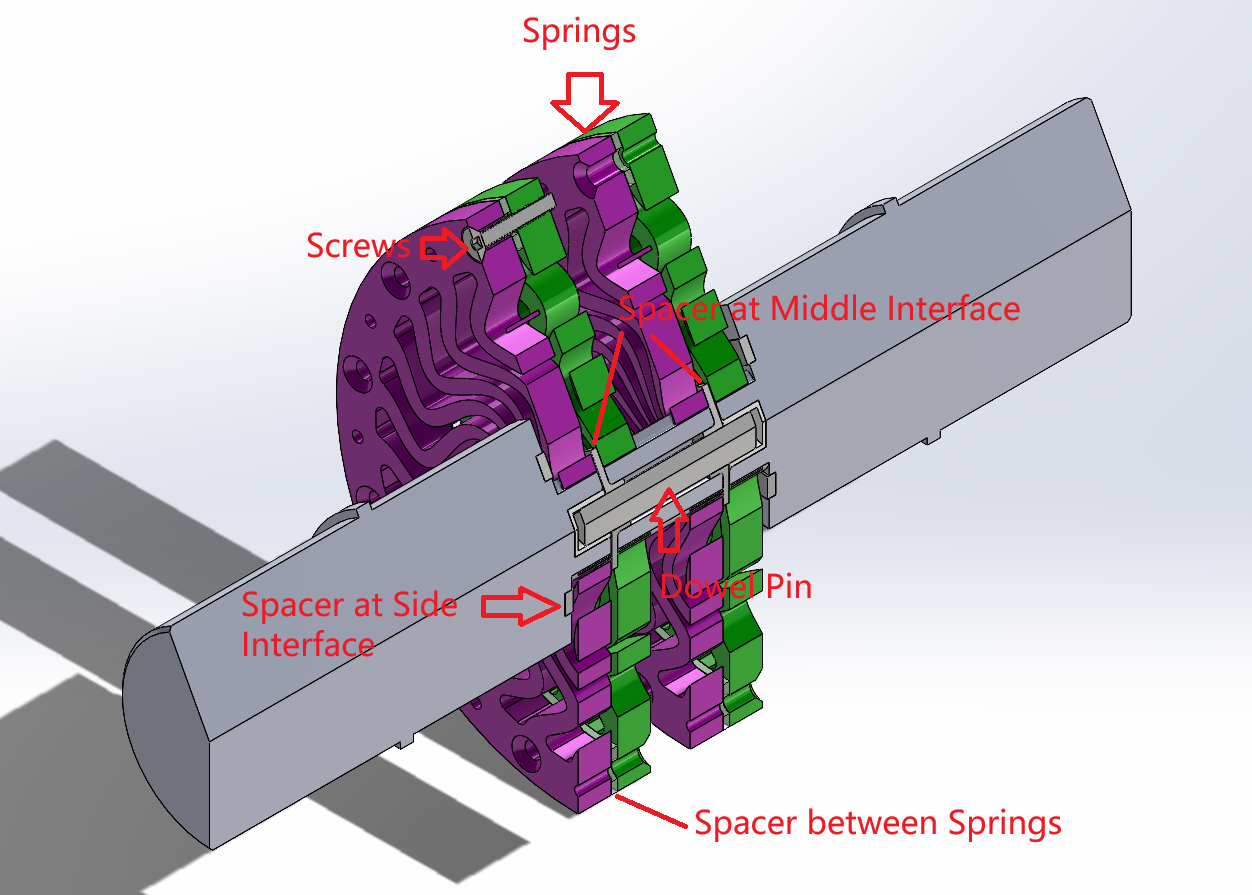
\includegraphics[width=0.45\textwidth]{portfolio/SeriesSpring_SectionView.png}
        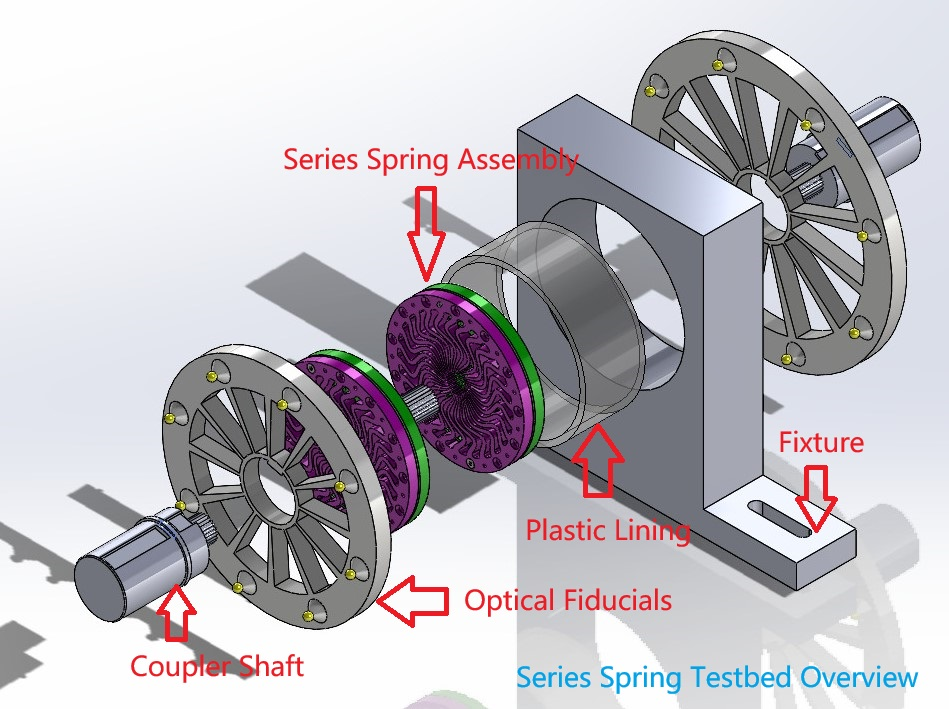
\includegraphics[width=0.45\textwidth]{portfolio/SeriesASSEM_4in1.JPG}
        \caption{CAD Design of Series Torsional Spring}
        \label{Series Spring CAD}

    \end{figure}

    \item {Measurement strategies and Noise Evaluation of flexure deflection of spring by computer vision, including masking, blurring \& grayscaling, and Hough Circle Transformation to recognize fiducial markers, as in Figure \ref*{Fiducials}. The center of the fiducial ring is determined by the triangular method.}
    \begin{figure}[H]

        \centering
        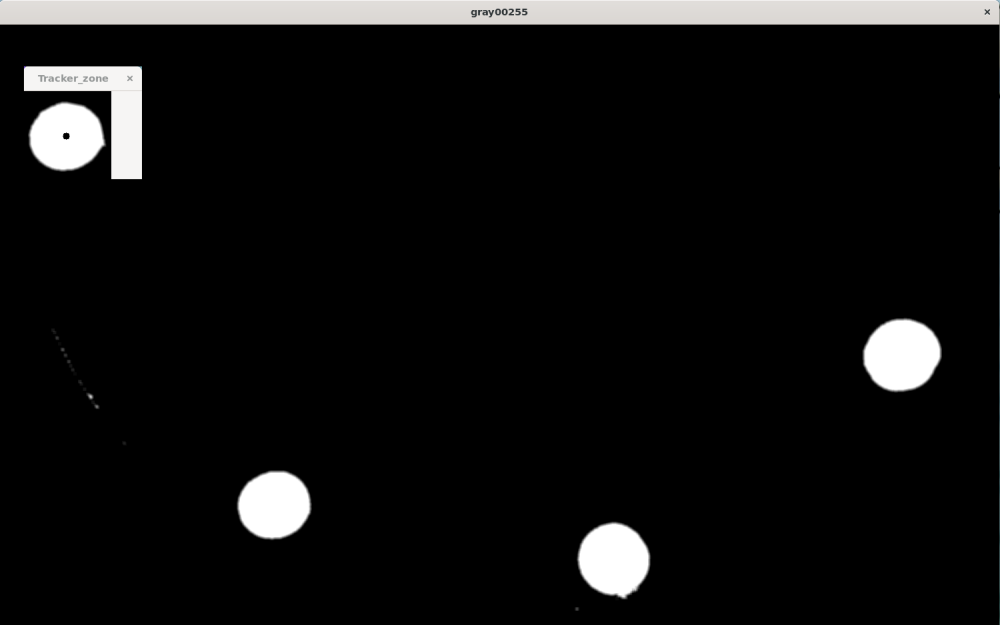
\includegraphics[width=0.45\textwidth]{portfolio/Blur_Gray.png}
        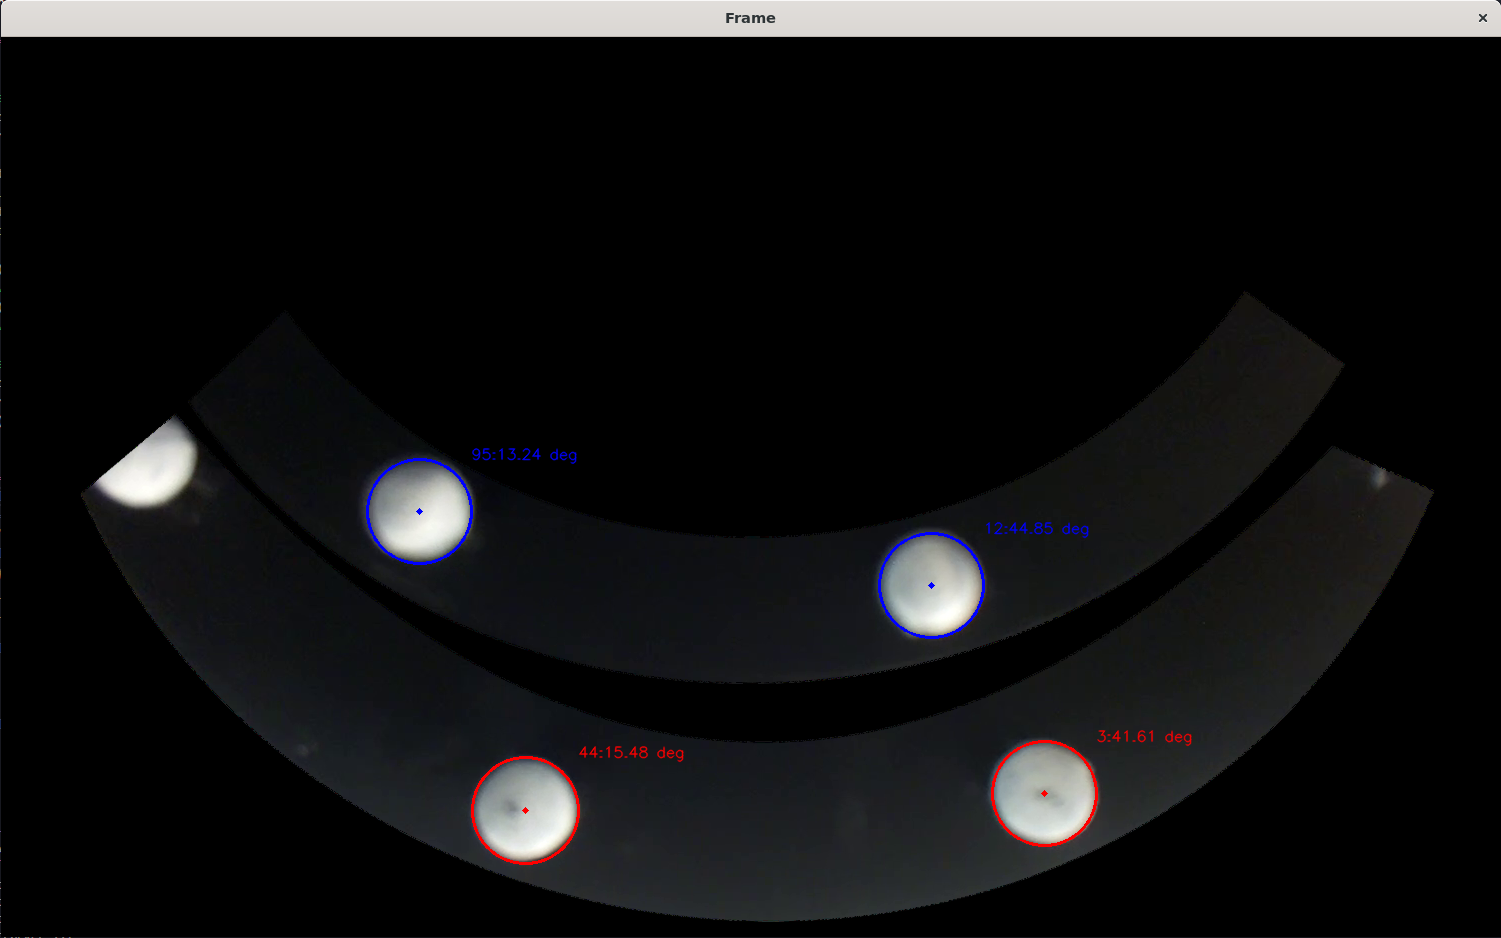
\includegraphics[width=0.45\textwidth]{portfolio/CircleAnnotate.png}
        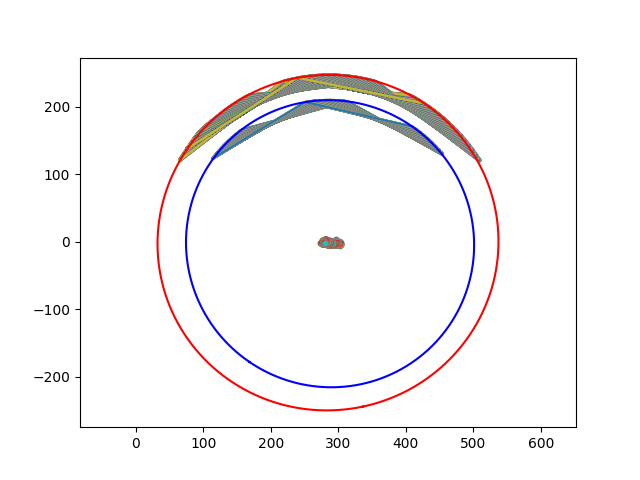
\includegraphics[width=0.45\textwidth]{portfolio/Center_Result.png}
        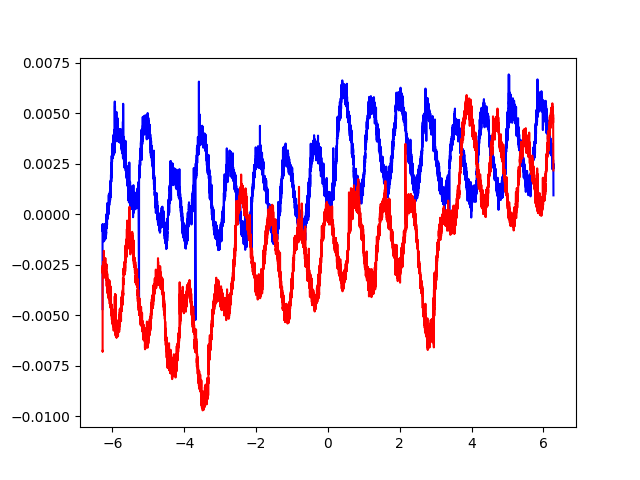
\includegraphics[width=0.45\textwidth]{portfolio/Noise_Eval.png}
        \caption{Fiducial Recognition and Deflection Angle Calculation}
        \label{Fiducials}

    \end{figure}

    \item {Evaluation of the measured stiffness of the series spring, as shown in Figure \ref*{Stiffness Measurement}.}
    \begin{figure}[H]

        \centering
        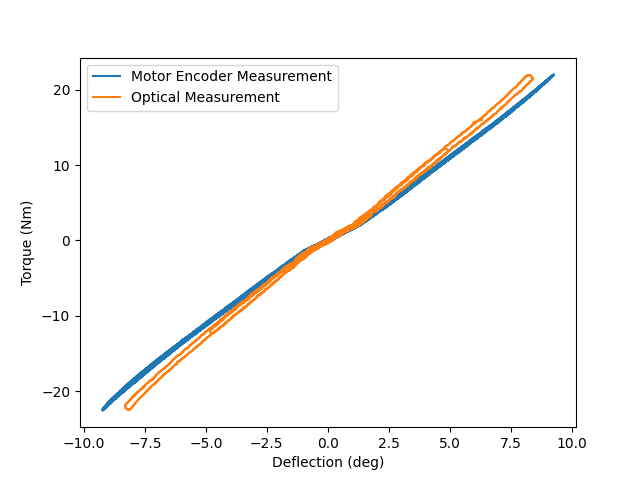
\includegraphics[width=0.7\textwidth]{portfolio/deflection_calc.png}
        \caption{Fiducial Recognition and Deflection Angle Calculation}
        \label{Stiffness Measurement}

    \end{figure}

\end{itemize}


% \begin{figure}

%     \centering
%     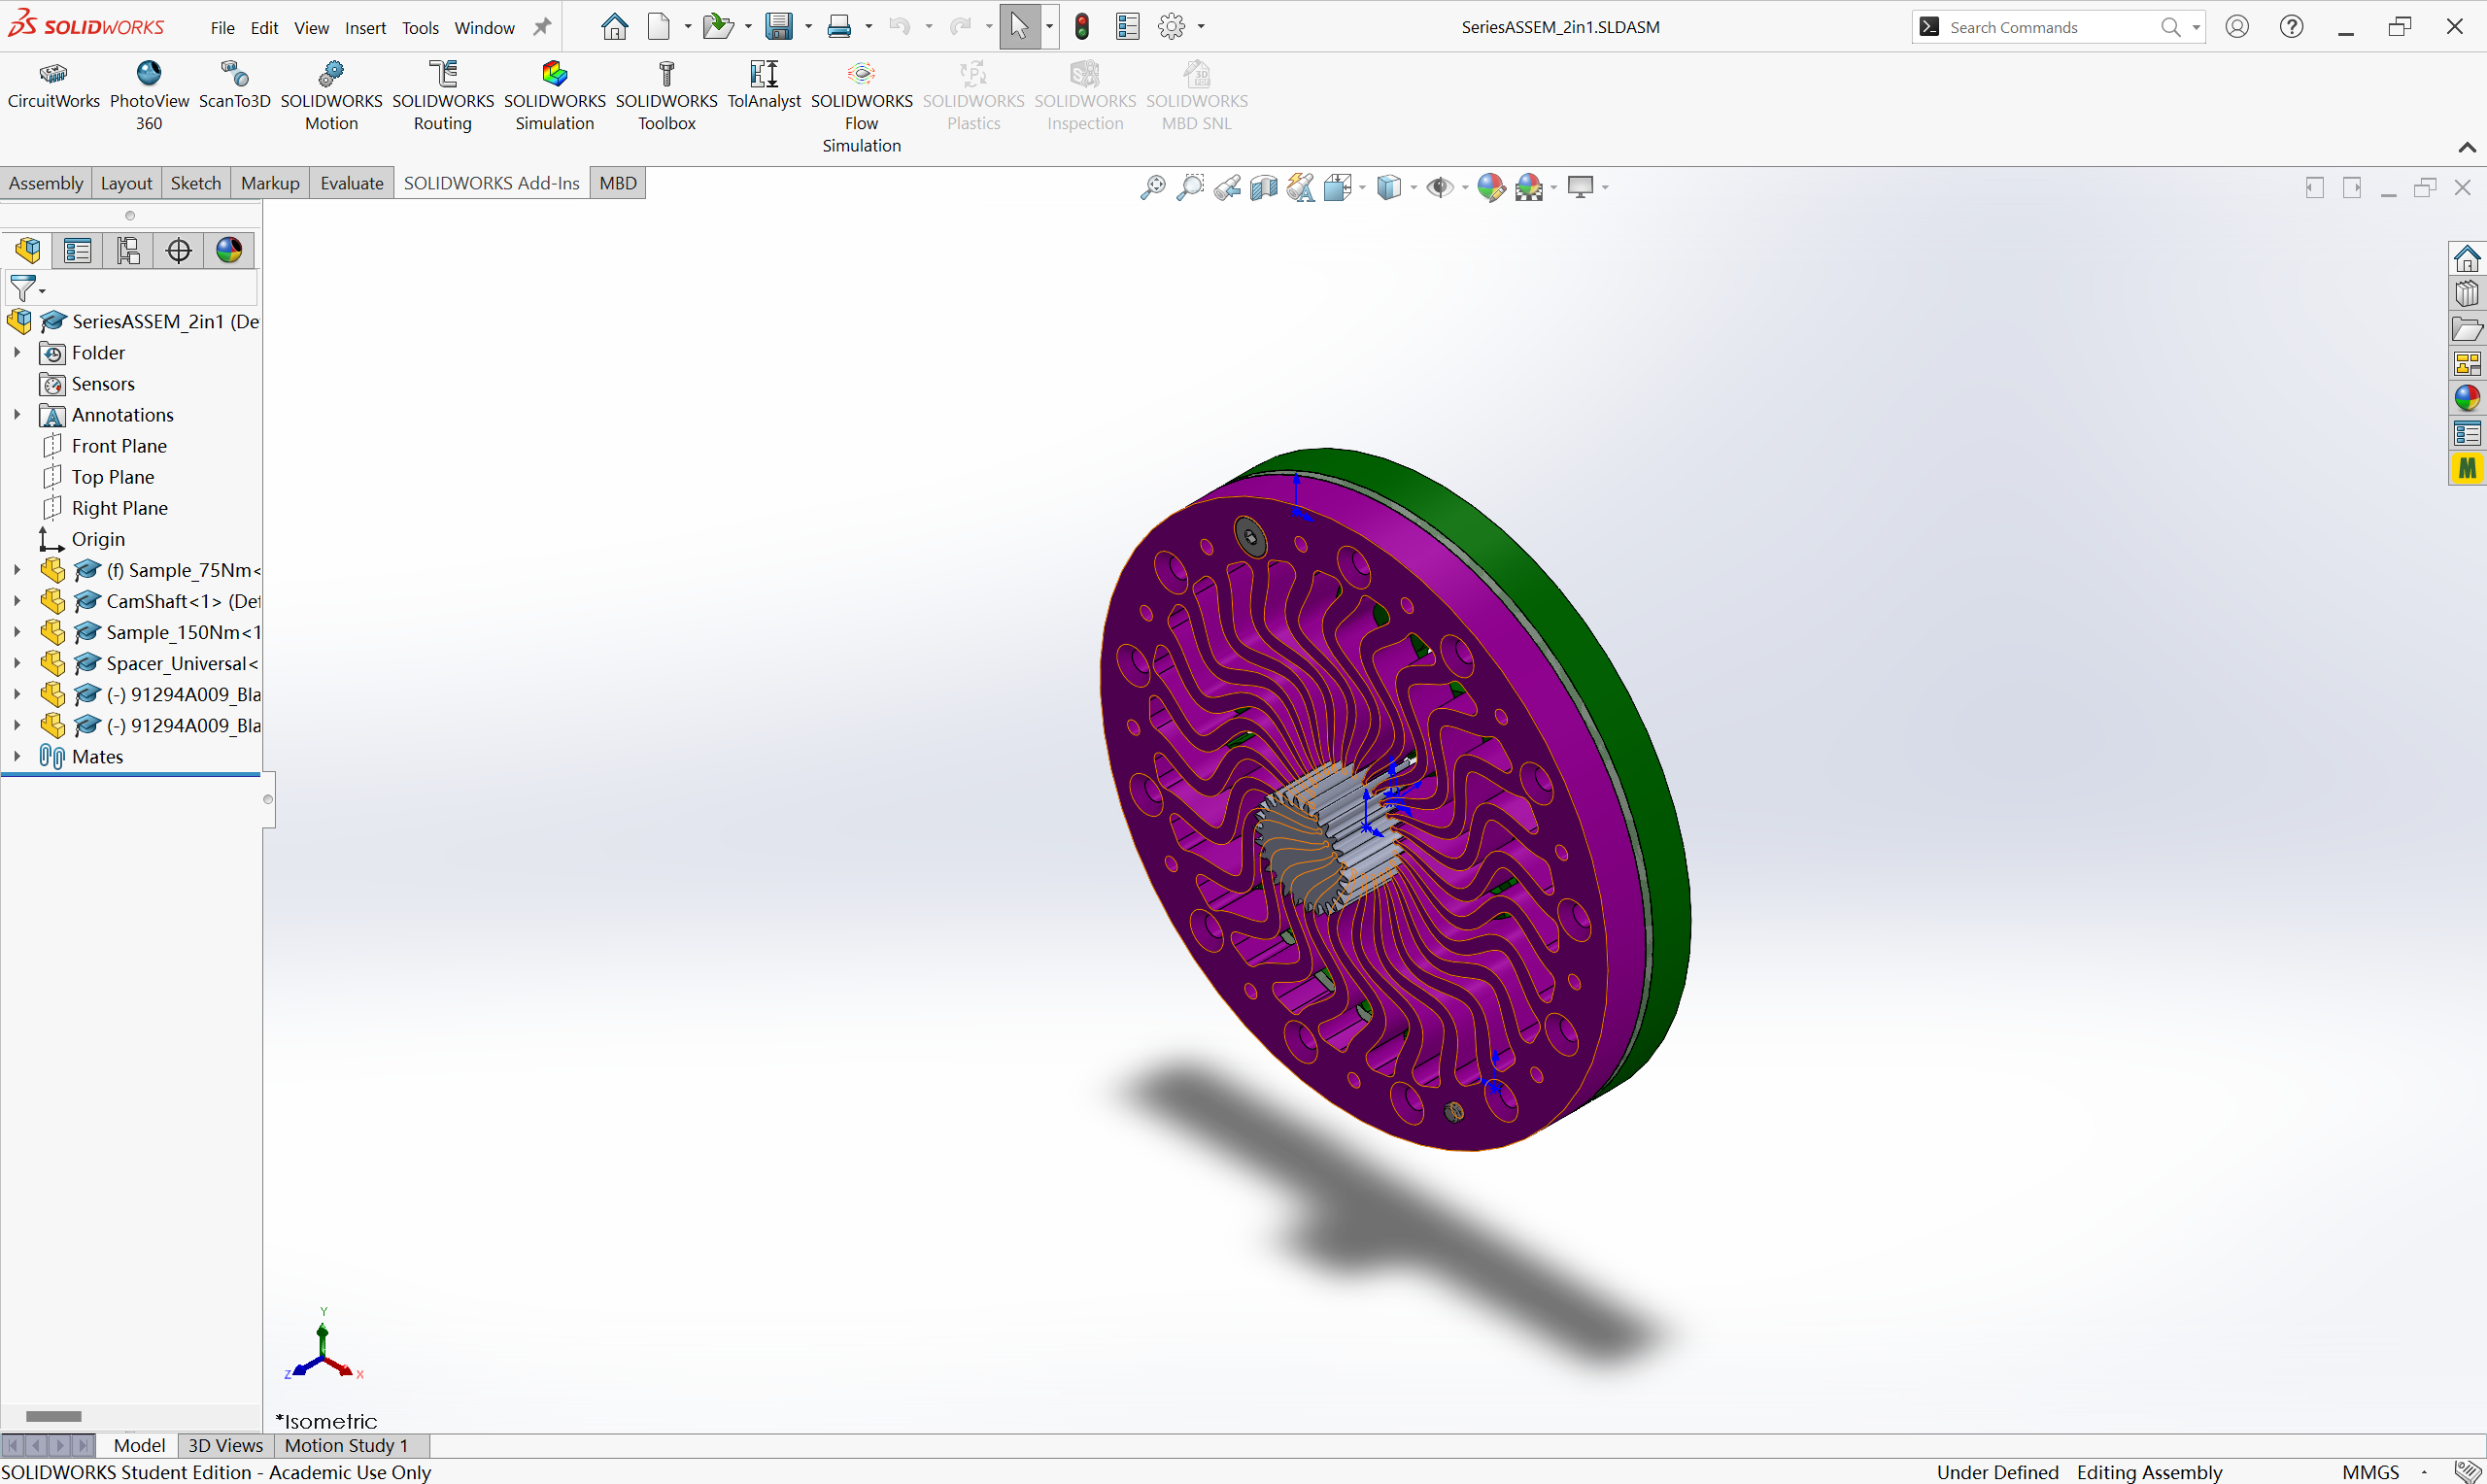
\includegraphics[width=1.0\textwidth]{portfolio/SeriesSpring_CAD.png}
%     \caption{CAD Design of Series Torsional Spring}
%     \label{Series Spring CAD}

% \end{figure}
\newpage

\section{Software Generalization for \href{https://www.opensourceleg.org/}{Open-Source Leg}}


\subsection{Background}

% -- BACKGROUND BEGINS -- % 


% WHAT IS OPENSOURCELEG
% -- DRAWNBACK / GAP: HOW / WHY IT IS NOT GENERALIZED ENOUGH -- %
The Open-Source Leg project is a standardized hardware and software platform for prosthesis designs, controls, and tests, aimed to eliminate the barriers among different prosthesis researches and serve as a bridge for collaborative efforts in prosthetic leg design and control. Such platform is expected to be flexible towards hardware choices. However, the previous versions of Open-Source Leg software library is biased to a specific hardware choice, which fails to close the gap between individual researches and adds difficulty in comparing experiment results. 

% -- MOTIVATION: A MORE GENERALIZED OPENSOURCELEG -- %
Thus, a generalized, user-friendly version of the software library is needed to serve as a basis for alternative prosthetic leg forks. Such library will allow other researchers to create their version of prosthetic leg with lower costs and more standardized features, in order to offer a common platform to test and evaluate further mechanical designs and control strategies.

% -- BACKGROUND ENDS -- % 

\subsection{Objectives}

\begin{enumerate}
    \item {Create a base library for Open-Source Leg actuator and sensor modules, to serve as a template for standardized development, with \href{https://github.com/neurobionics/opensourceleg}{merged into GitHub Repo}.}
    \item {Redevelop the instance of actuator modules based on the generalized library design.}
    \item {Test and compare the performance of different actuators and sensors based on the generalized library design.}
\end{enumerate}

\subsection{Results}


\begin{itemize}

    \item{A base library for Open-Source Leg actuator and sensor modules, as Figure \ref*{Python Lib Class Diagram}, and examples of a redeveloped actuator module.}
    
    \begin{figure}[H]
        \centering
        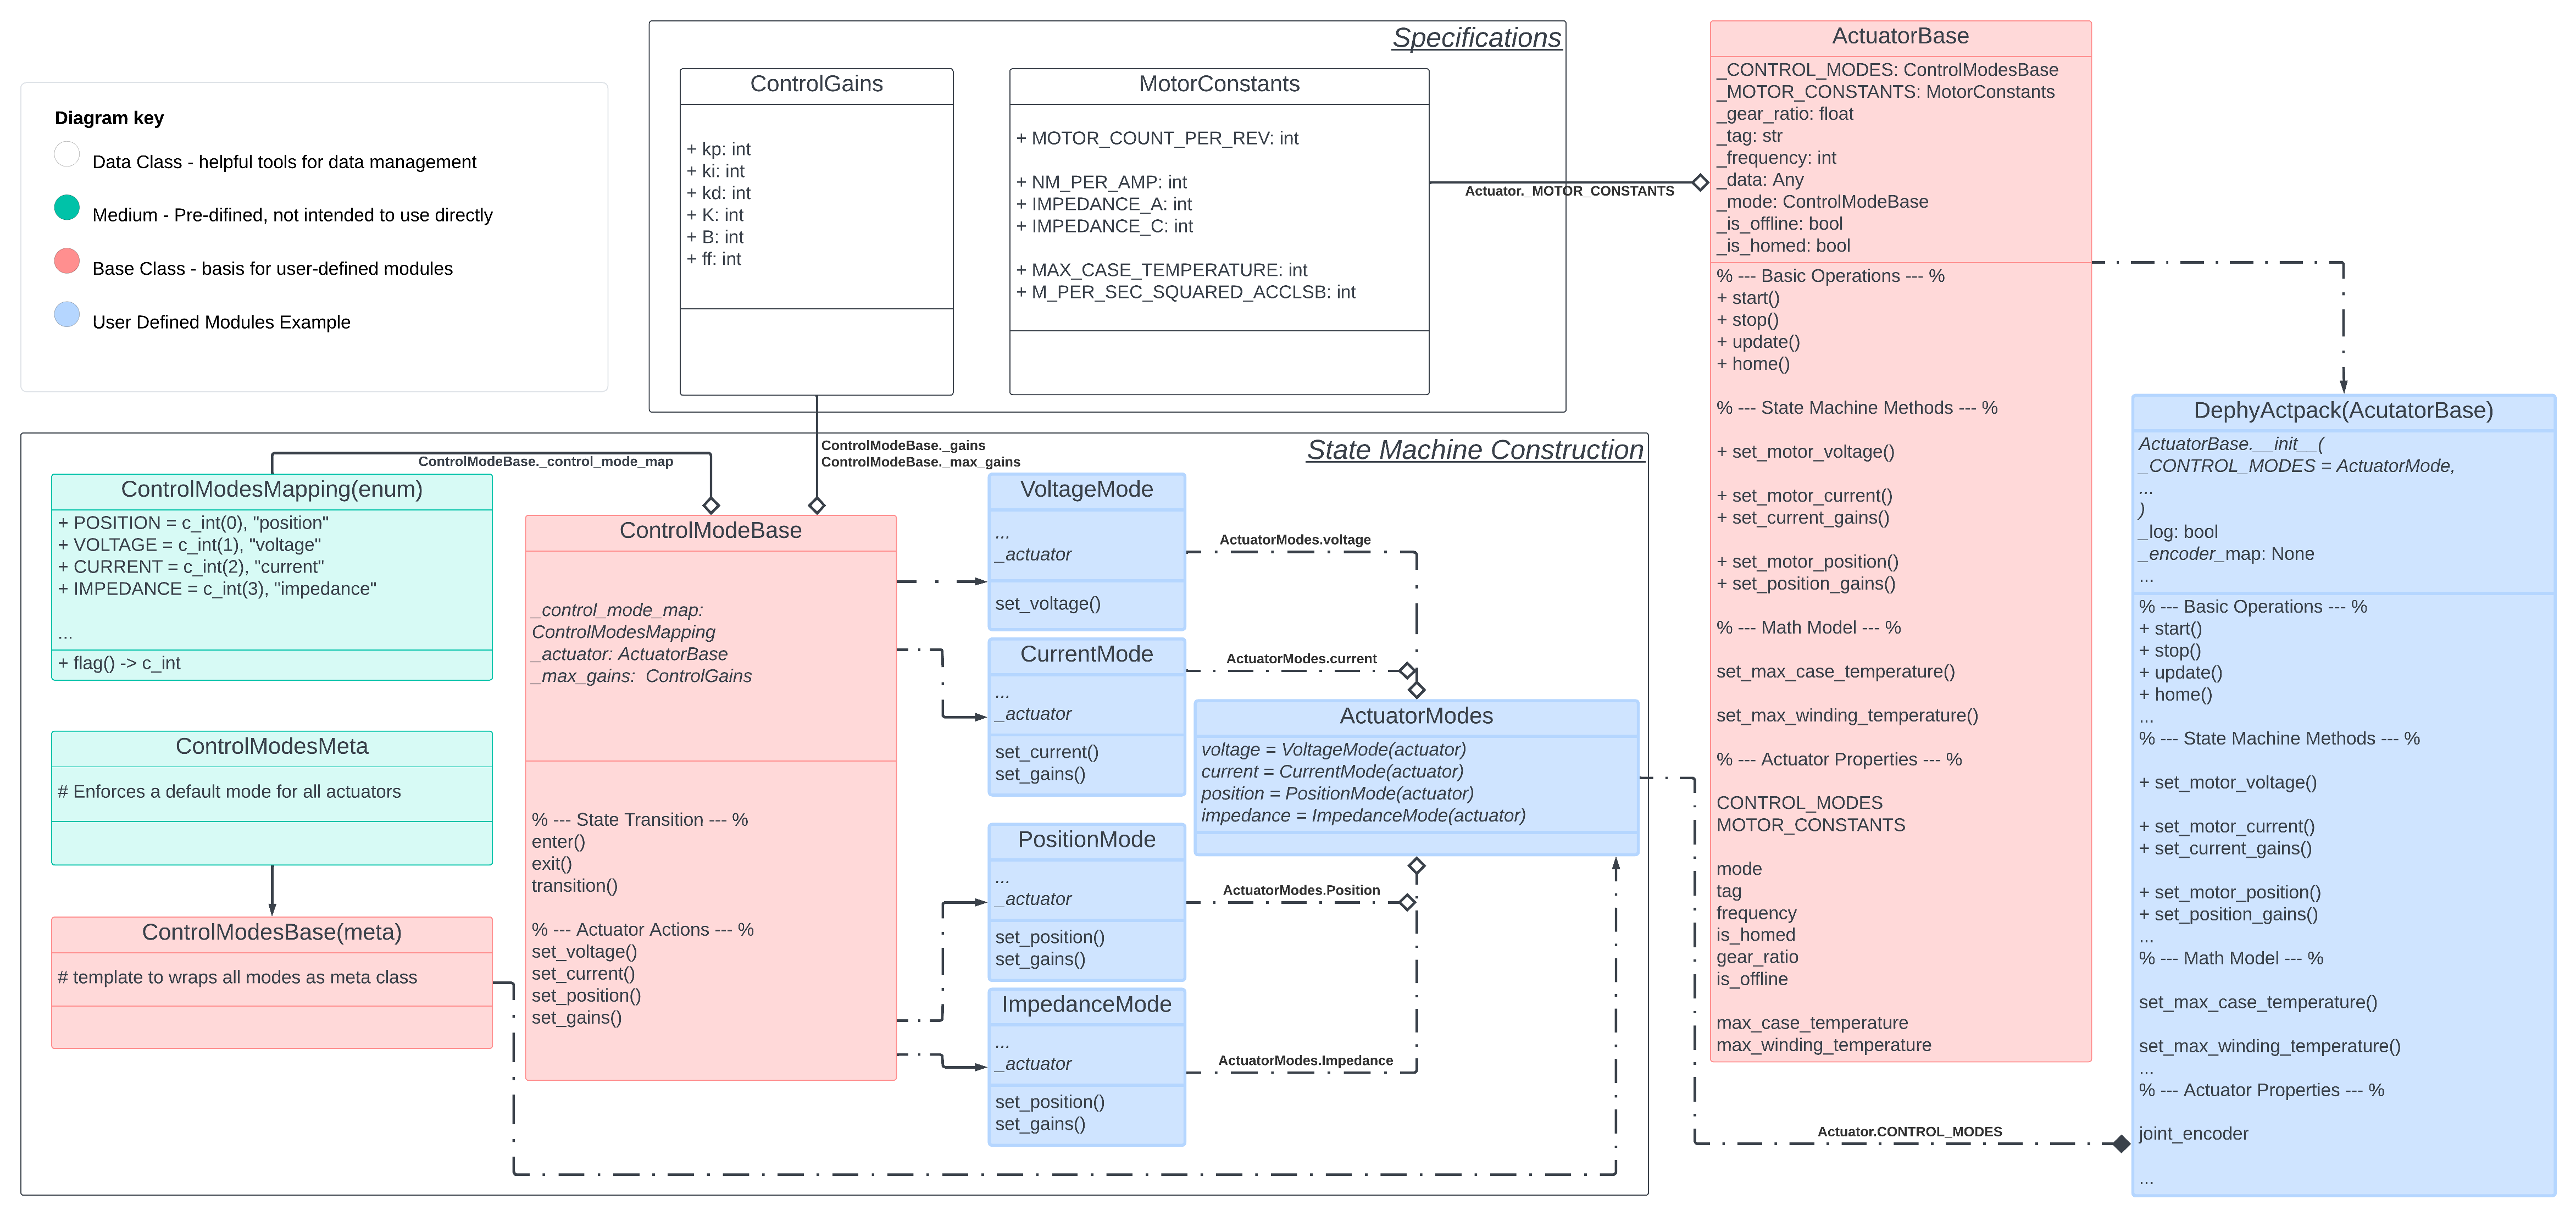
\includegraphics[width=1.0\textwidth]{portfolio/Class Diagram Base Lib.png}
        \caption{Class Diagram of Generalized Python Library}
        \label{Python Lib Class Diagram}
    \end{figure}
    \item {Performance evaluation across different actuator choices, as Figure \ref{Dephy-Moteus Comp}}
    
    \begin{figure}[H]
        \centering
        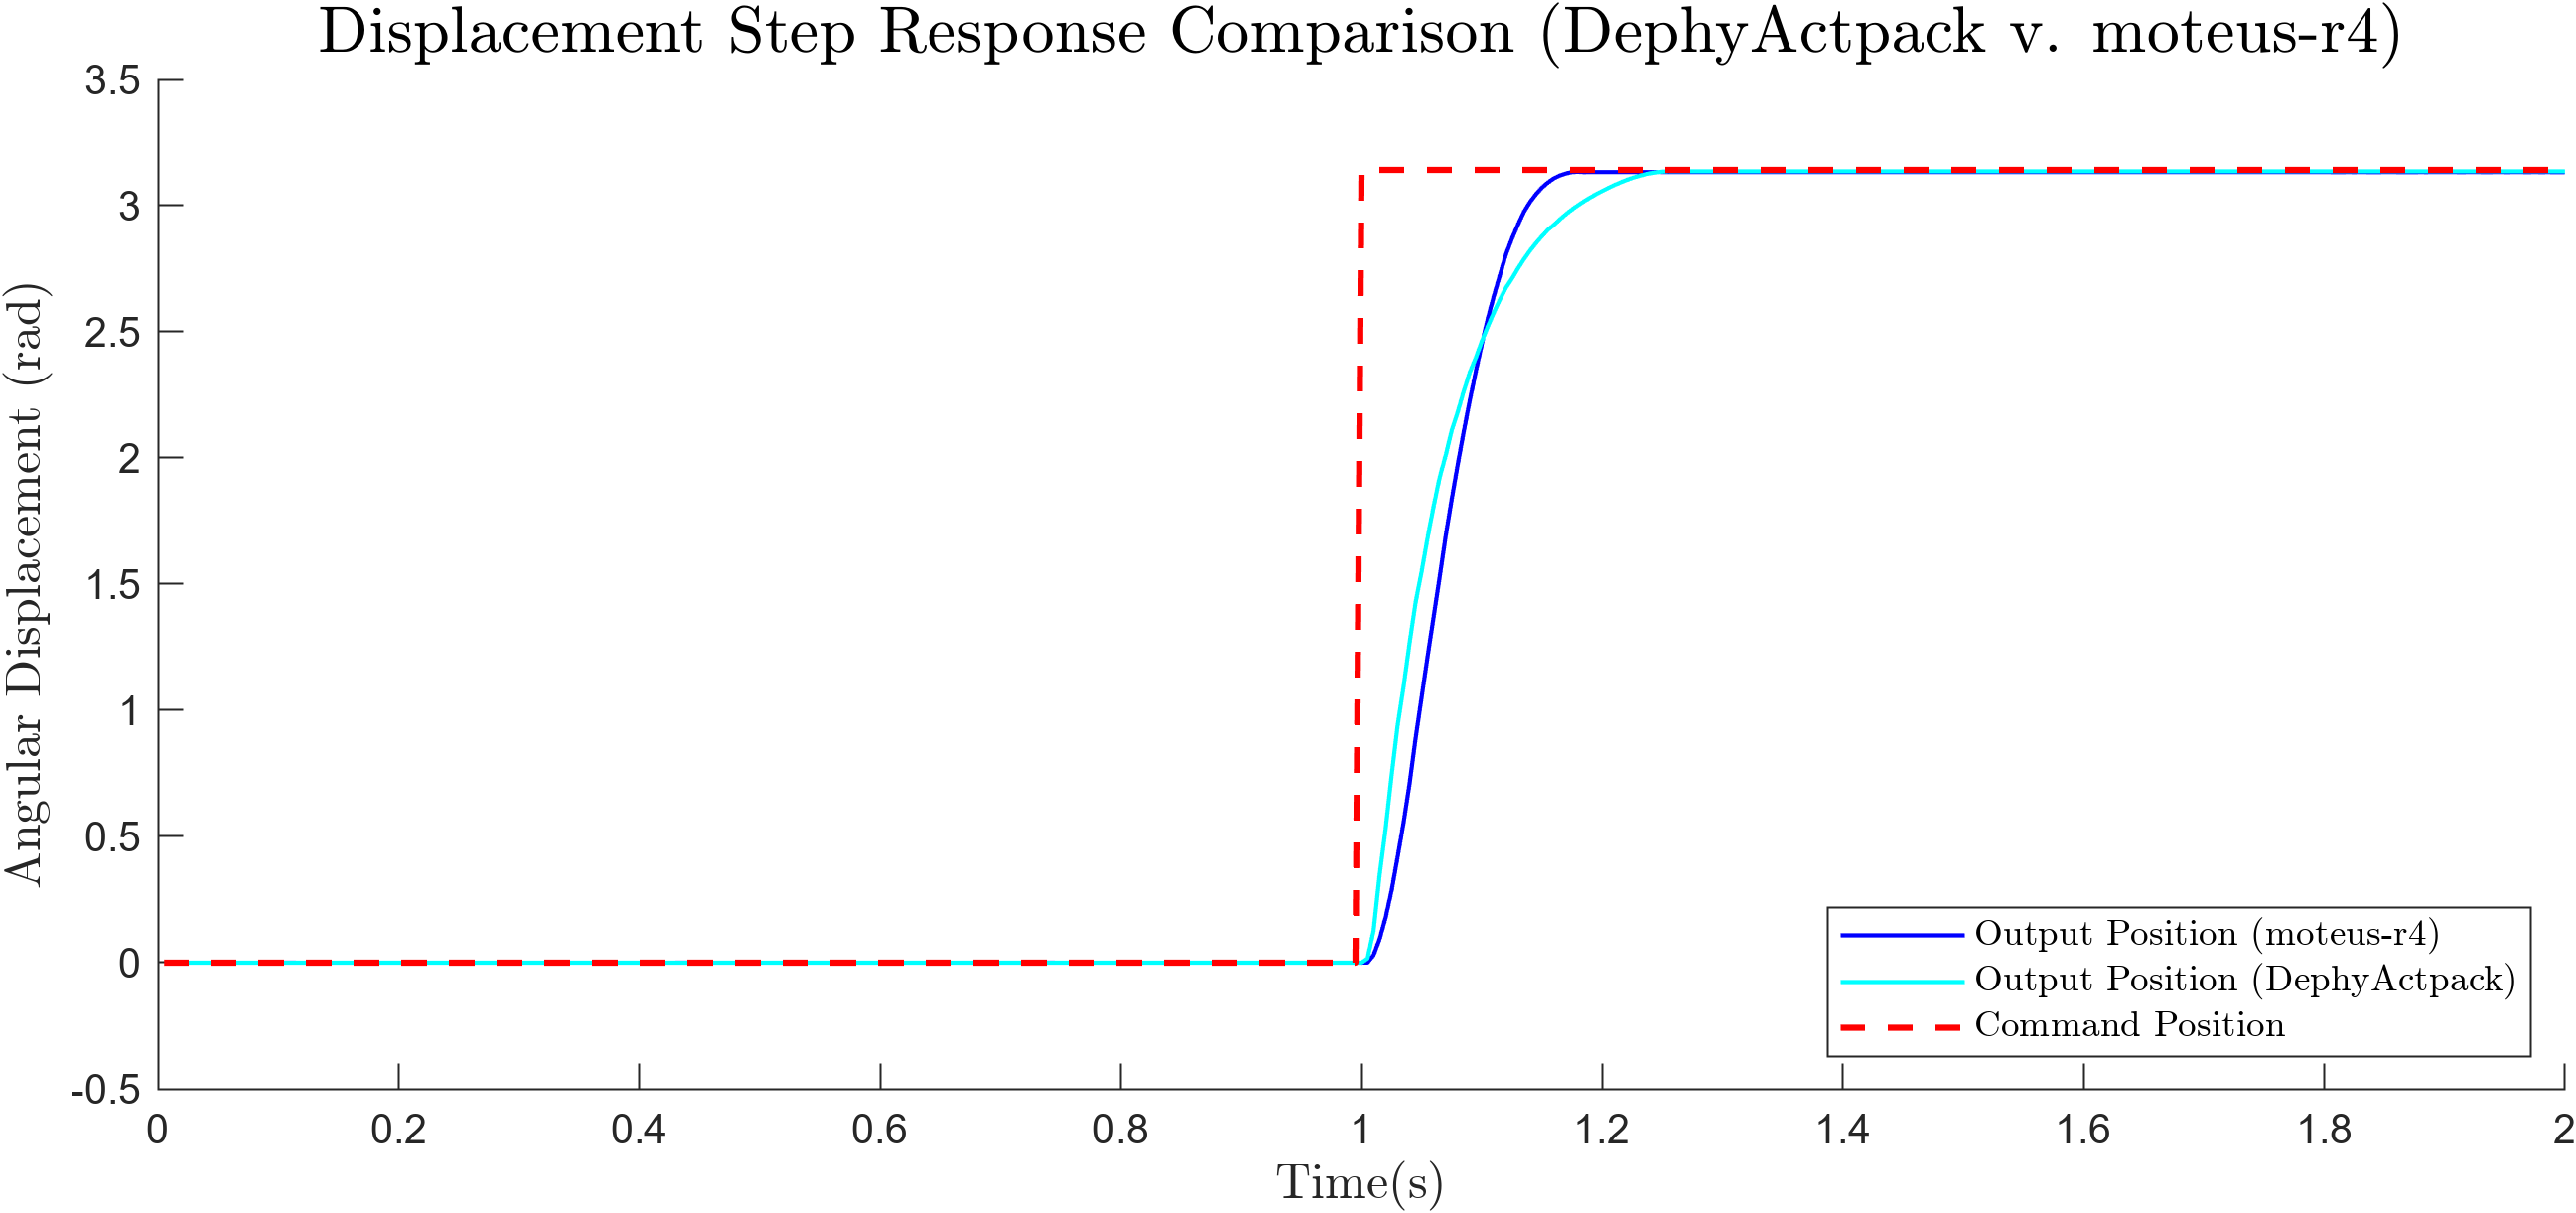
\includegraphics[width=0.6\textwidth]{portfolio/position_comp.png}
        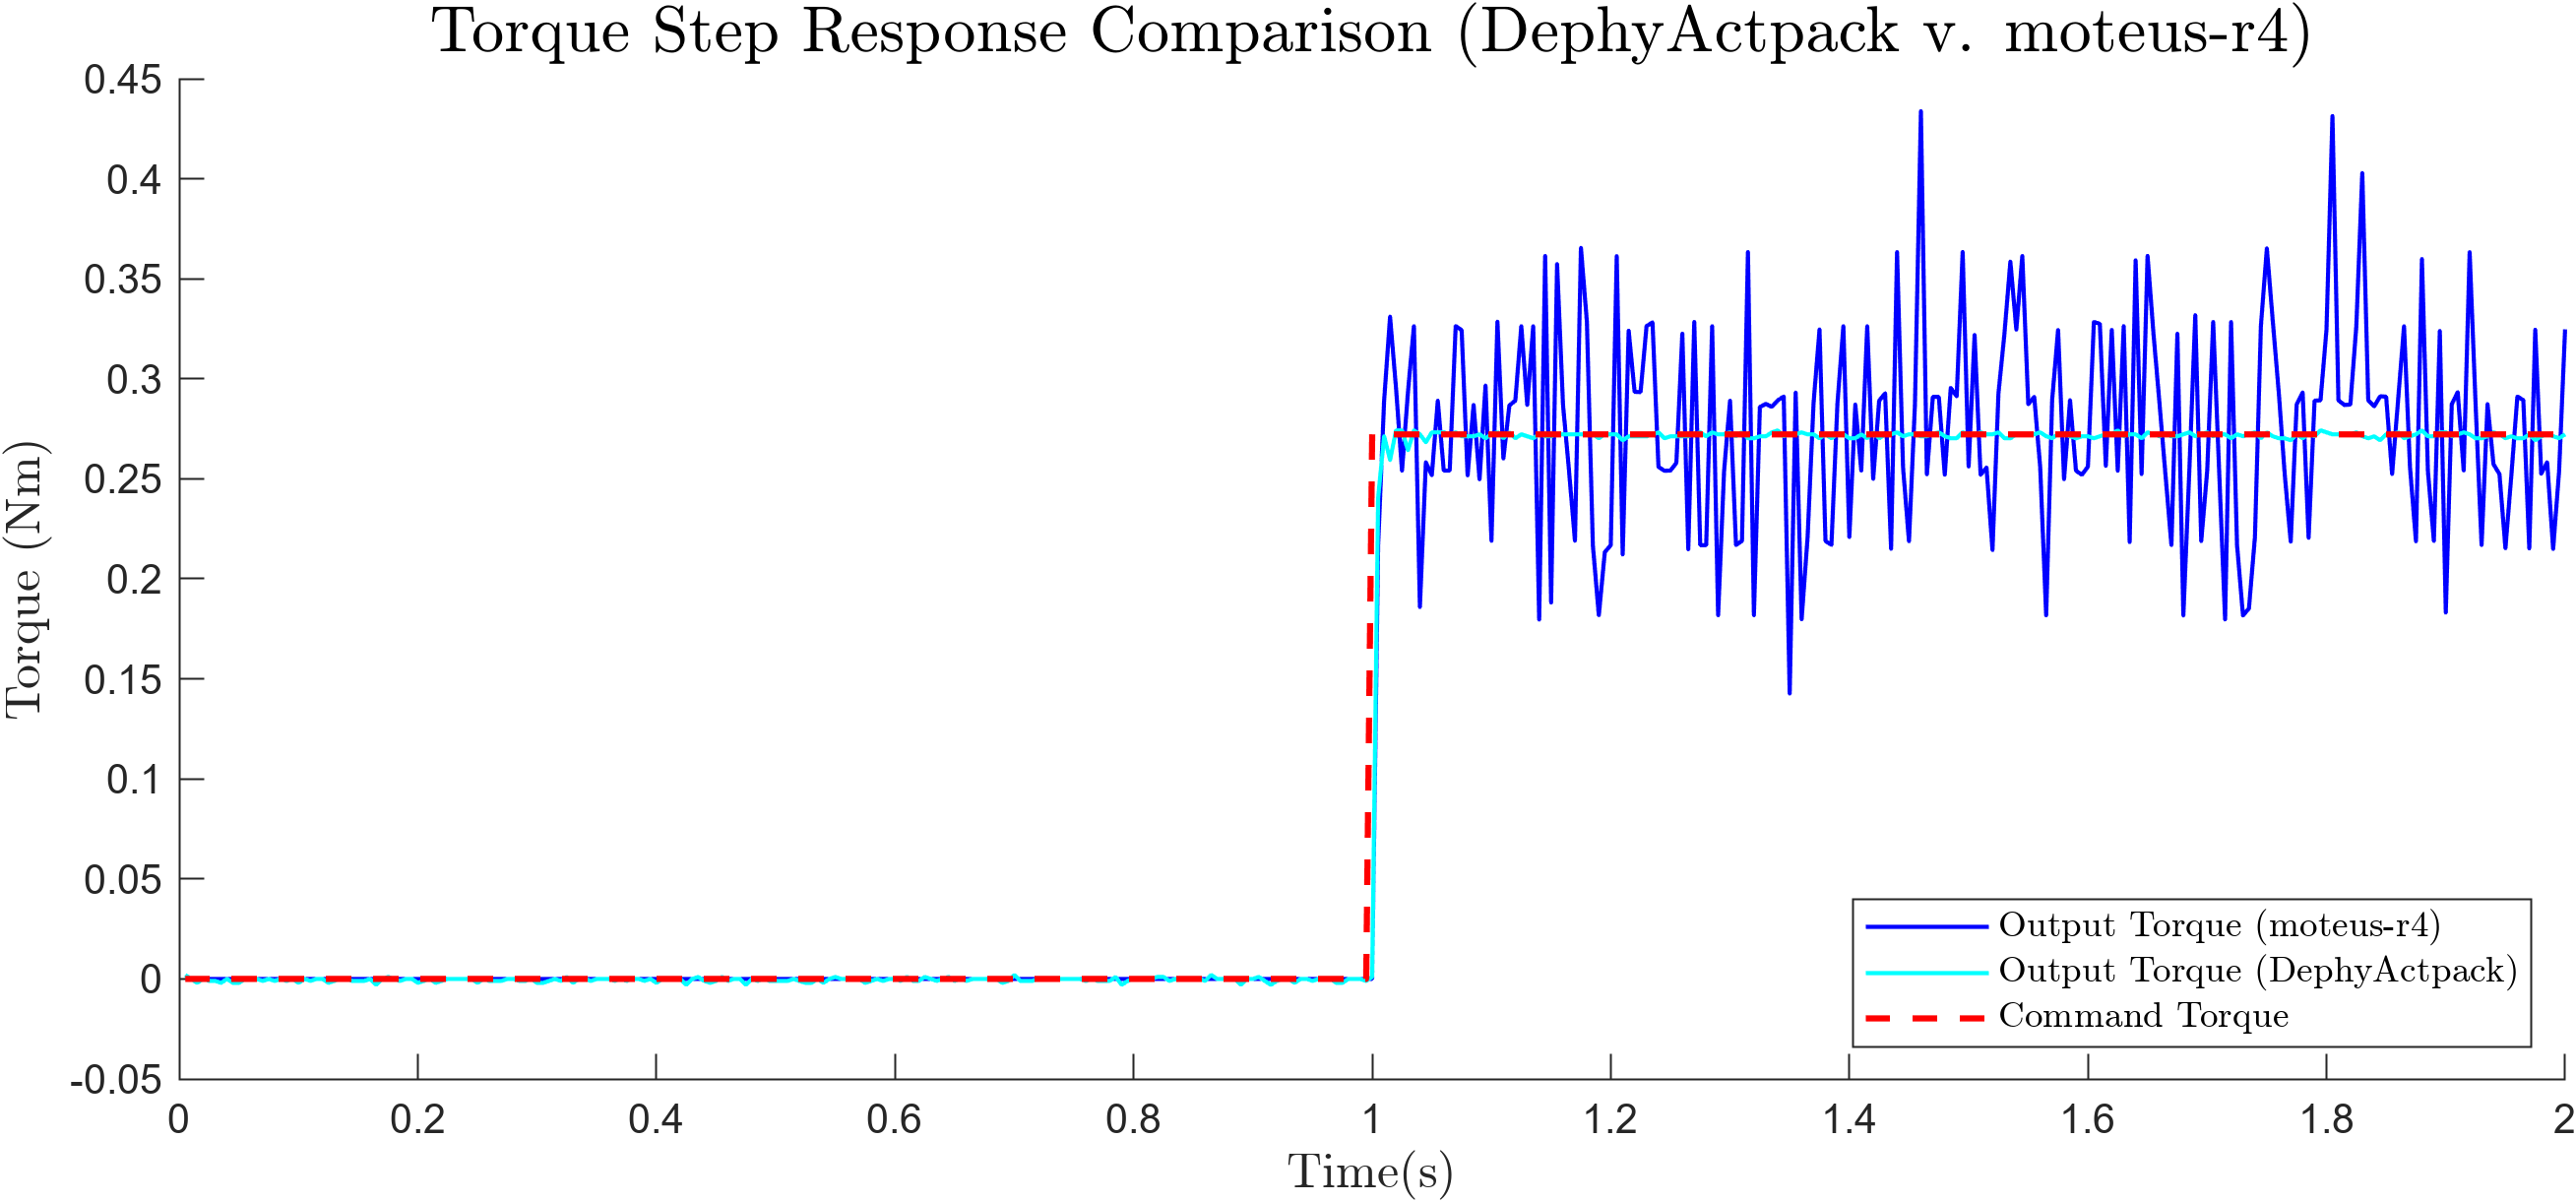
\includegraphics[width=0.6\textwidth]{portfolio/torque_comp.png}
        \caption{Performance Evaluation \& Comparison of Different Actuators on Generalized Library}
        \label{Dephy-Moteus Comp}
    \end{figure}
    

\end{itemize}

\newpage

\section{Motion Analysis \& Design of Robot Swimmer Model}


\subsection{Background}

Targeting transport is an emerging field in the medical industry that is attempting to obtain a more precise cure for the diseased area in the human body. Although attempts such as targeted therapy are performed, they still inherits the same problem that both the location and the amount of optimal dosing are hard to be controlled. 

Therefore, a complete robot swimmer model should be developed to perform the task, due to its better performance than chemical-based therapies. Such design aims to offer a feasible solution for future research in control strategies for robot swimmers, in order to achieve better performances in targeting transportation. 


\subsection{Objectives}

\begin{enumerate}
    
    \item {Develop a mechanical model with sphere head and flagella (as a mimic of bacteria with dual flagella), and the corresponding kinematics model, that is suitable to perform object tracking.}
    \item {Evaluate the design \& control strategies from computational simulations. }
    
\end{enumerate}

\subsection{Results}

\begin{enumerate}

    \item {Mechanical Design of the Components of Robot Swimmer, with Computational Fluid Dynamics (CFD) analysis to validate the design, as shown in Figure \ref*{Design-RobotSwimmer}. }
    
    \begin{figure}[H]
        \centering
        \includegraphics*[width = 0.7\textwidth]{portfolio/overview new.png}
        \caption{Mechanical Design of Robot Swimmer}
        \label{Design-RobotSwimmer}
    \end{figure}
    
    \item {Kinematics Analysis of the Robot Swimmer Model, as shown in Figure \ref*{FBD-RobotSwimmer}.}
    
    \begin{figure}[H]
        \centering
        \includegraphics*[width = 0.5\textwidth]{portfolio/FBD_RobotSwimmer.png}
        \caption{Free Body Diagram of Robot Swimmer Model}
        \label{FBD-RobotSwimmer}
    \end{figure}

    \item {Control strategies applied to the Robot Swimmer Model (Feedback Control \& Feedforward Control, as in Figure \ref{Control-Blockdiagram}), with performance evaluation in simulations, as shown in Figure \ref{Control-RobotSwimmer}.}

    \begin{figure}[H]
        \centering
        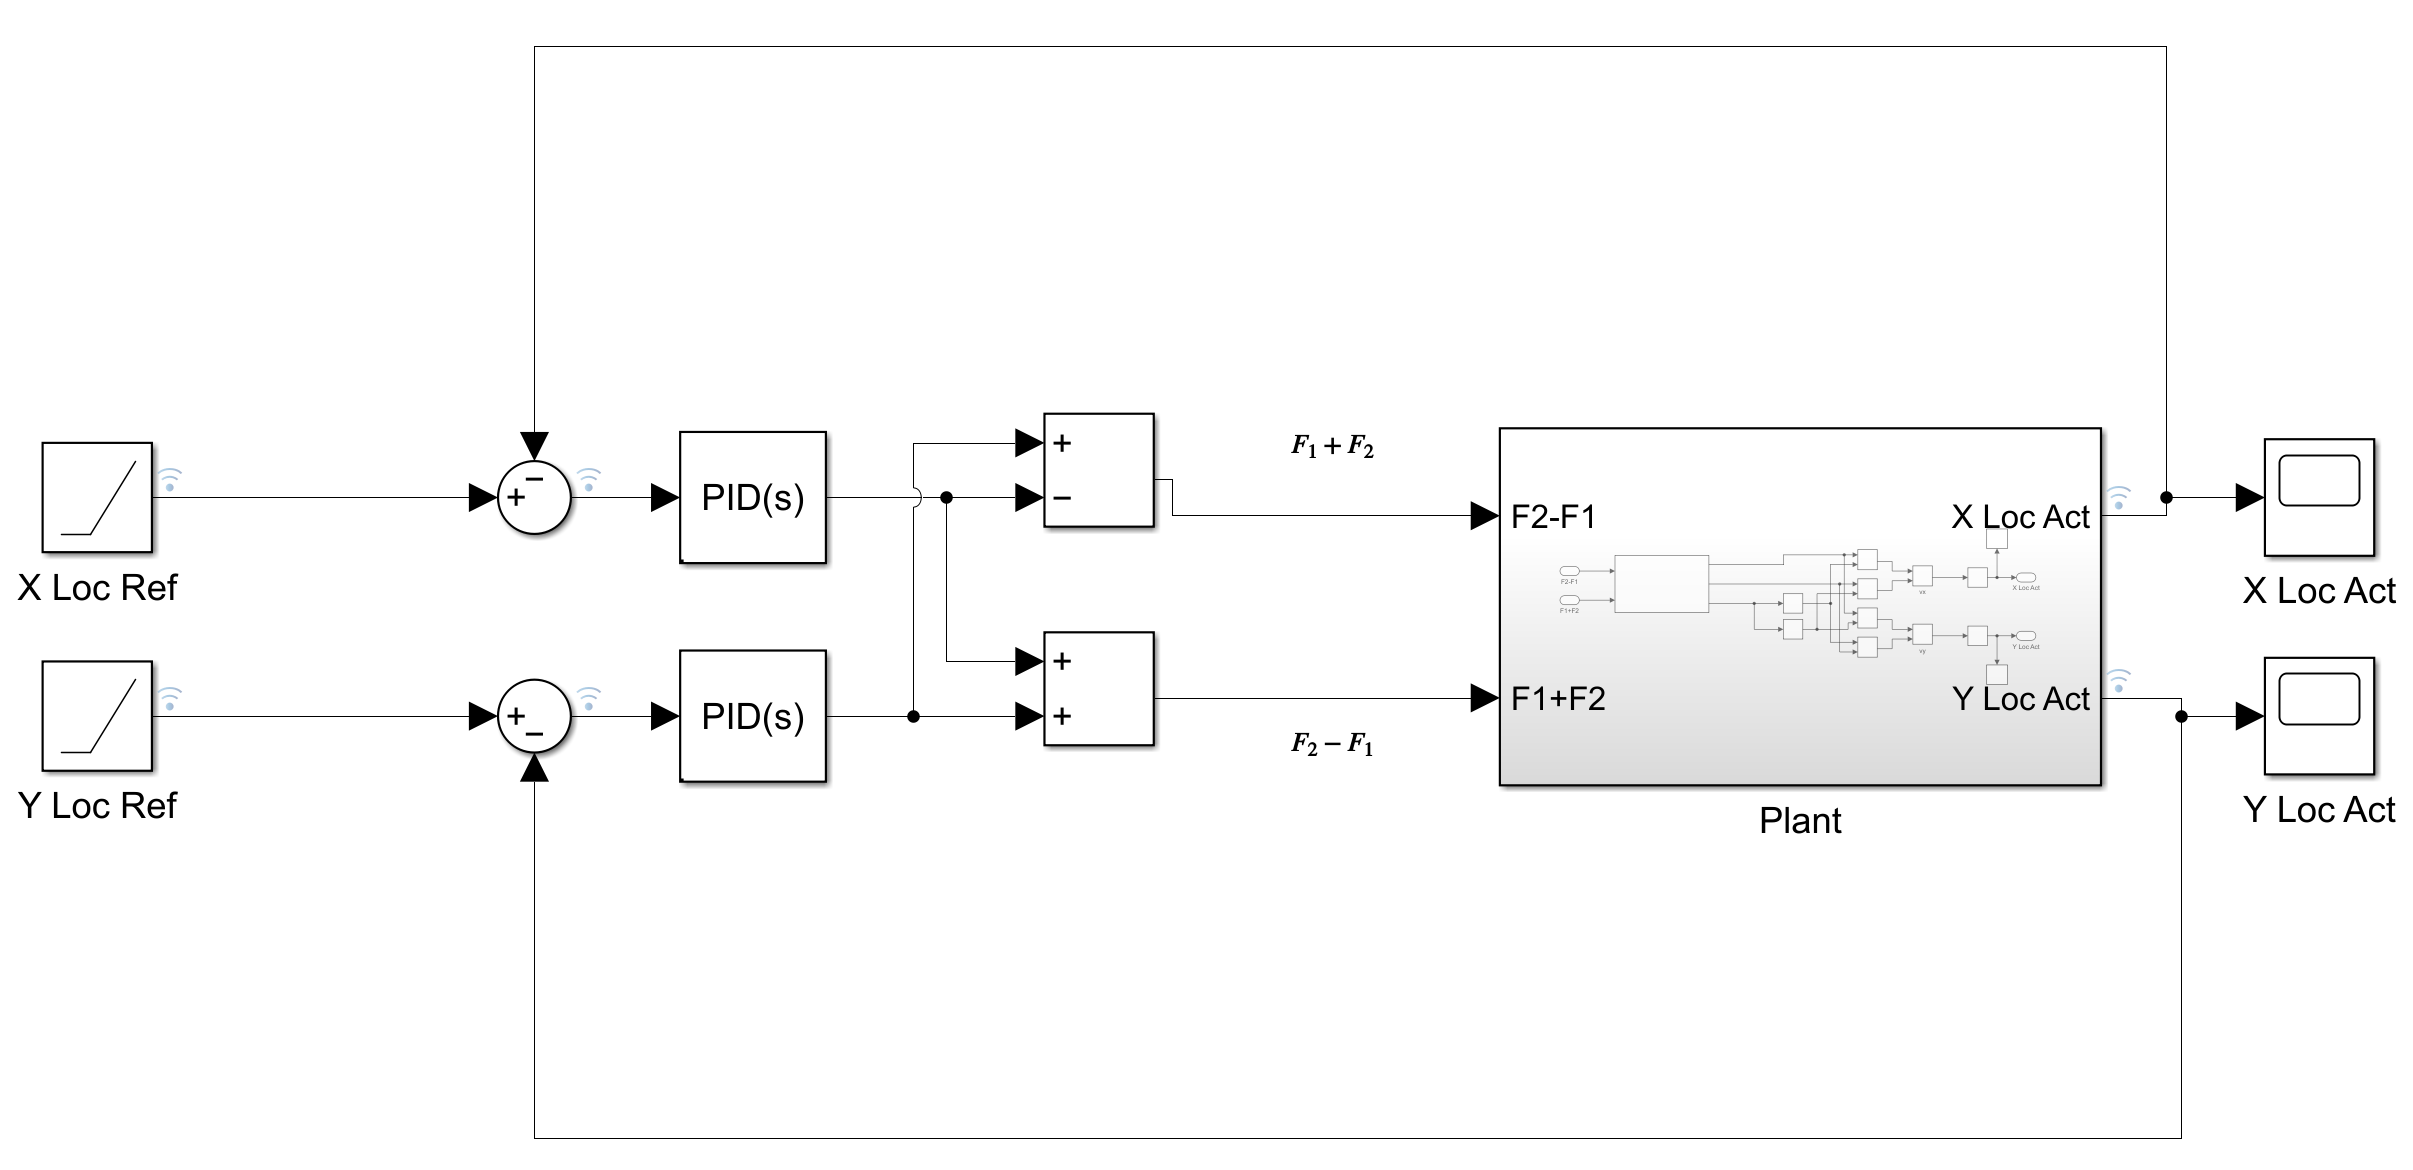
\includegraphics[width=0.9\textwidth]{portfolio/Robot_ClosedLoop.png}
        \caption{Modelling of Feedback Controller as Block Diagram}
        \label{Control-Blockdiagram}
    \end{figure}

    \begin{figure}[H]
        \centering
        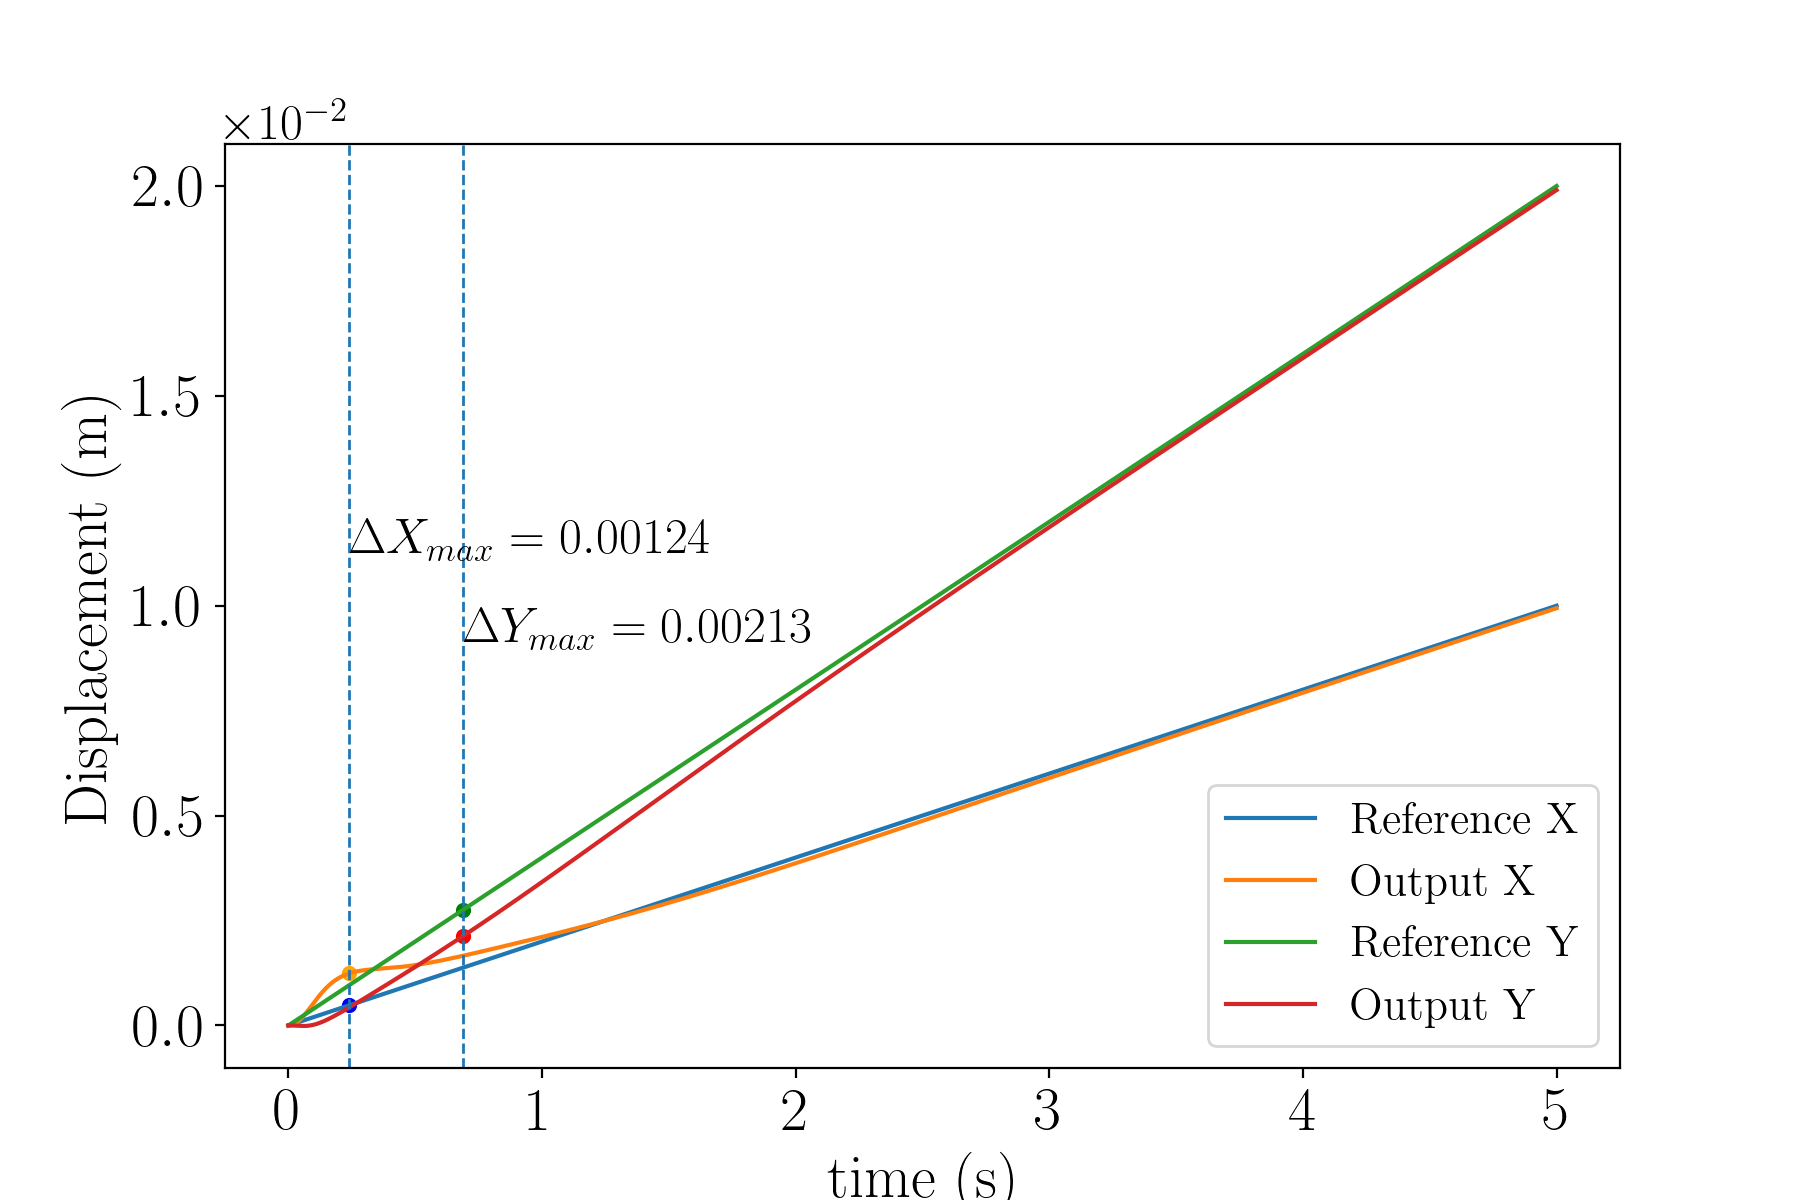
\includegraphics[width=0.45\textwidth]{portfolio/fig01_TrackingBehavior.png}
        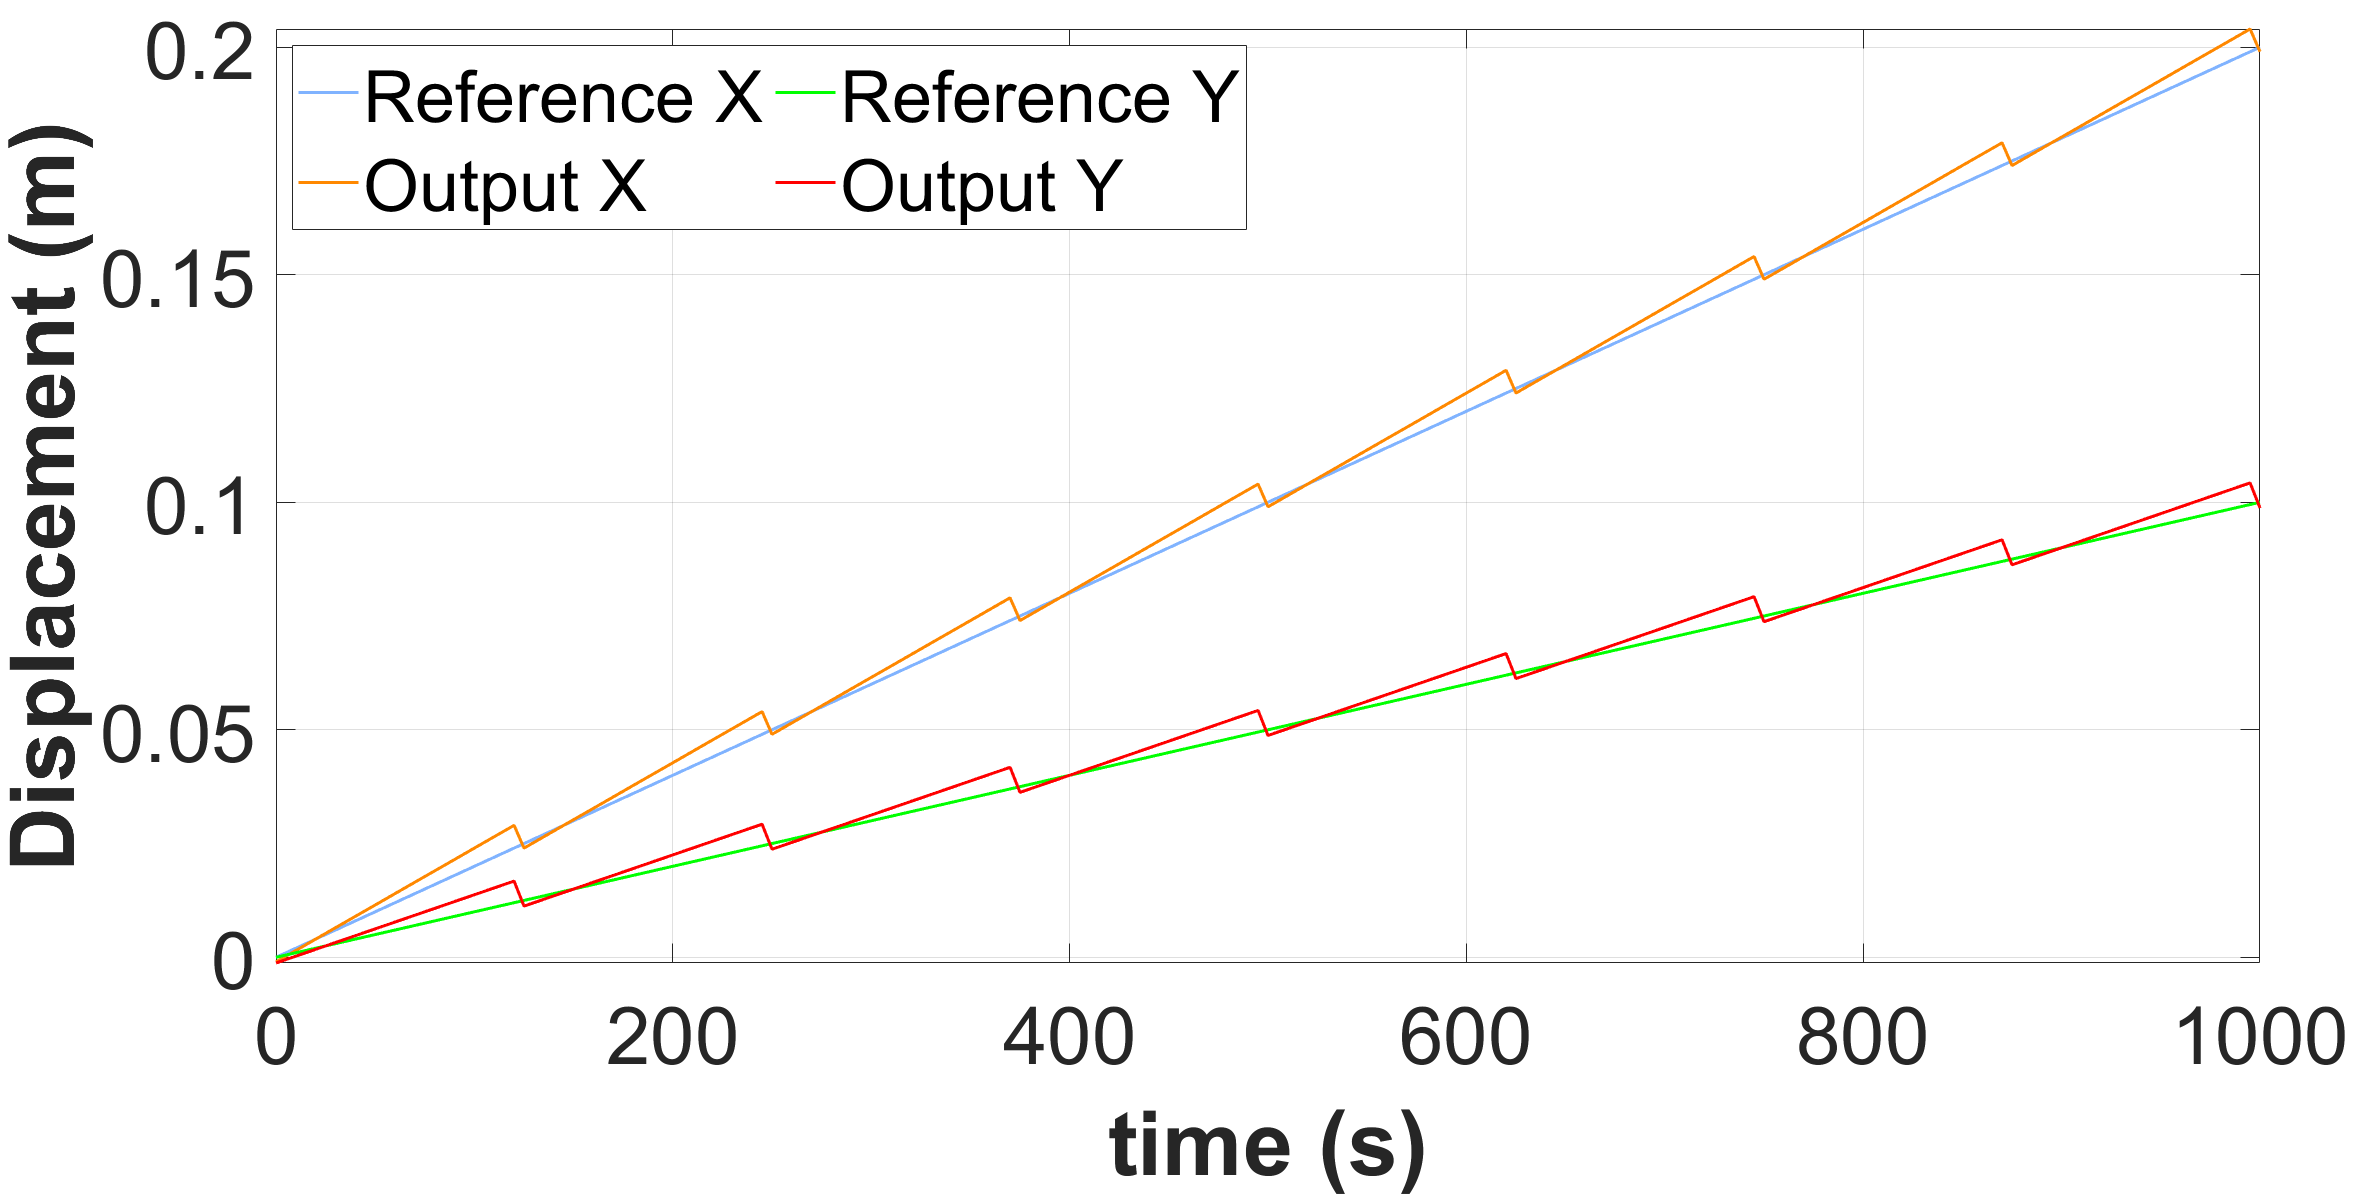
\includegraphics[width=0.45\textwidth]{portfolio/feedforward_track.png}
        \caption{Performance Evaluation of Tracking Behavior Under Different Control Strategies}
        \label{Control-RobotSwimmer}
    \end{figure}
    
\end{enumerate}

\newpage



\section{Classification Model for Heart Disease Diagnosis}


\subsection{Background}

Due to the increase probability to get heart diseases, the hospital is experiencing more and more pressure from the cardiovascular department. The idea to develop a classification model comes up correspondingly, to reduce the heavy burden from the diagnostics side. Such model is expected to classify different kinds of heart diseases, predict the probability of having heart diseases when given the specifications of one's health status, and  

\subsection{Objectives}

\begin{enumerate}

    \item{\small Work on diagnostic data of cardiac patients through feature selection}
    \item{\small Develop regression models (e.g., Random Forest) via Scikit-Learn and PyTorch in Python and use training data sets of clinical diagnostic data}
    \item{\small Test model performance on internal datasets}
    \item{\small Perform interpretability analysis of built models using variable sensitivity analysis}
    \item{\small Enhance classification processes' precision of the model by analyzing visualized Decision Trees}

\end{enumerate}

\subsection{Results}

\begin{itemize}

    \item{A random forest classification model to classify and predict heart diseases, as shown in \ref*{Random Forest Model}. Model posted as \href{https://github.com/Robin0265/HeartDisease_Regression}{GitHub Repo}.}
    
    \begin{figure}[H]
        \centering
        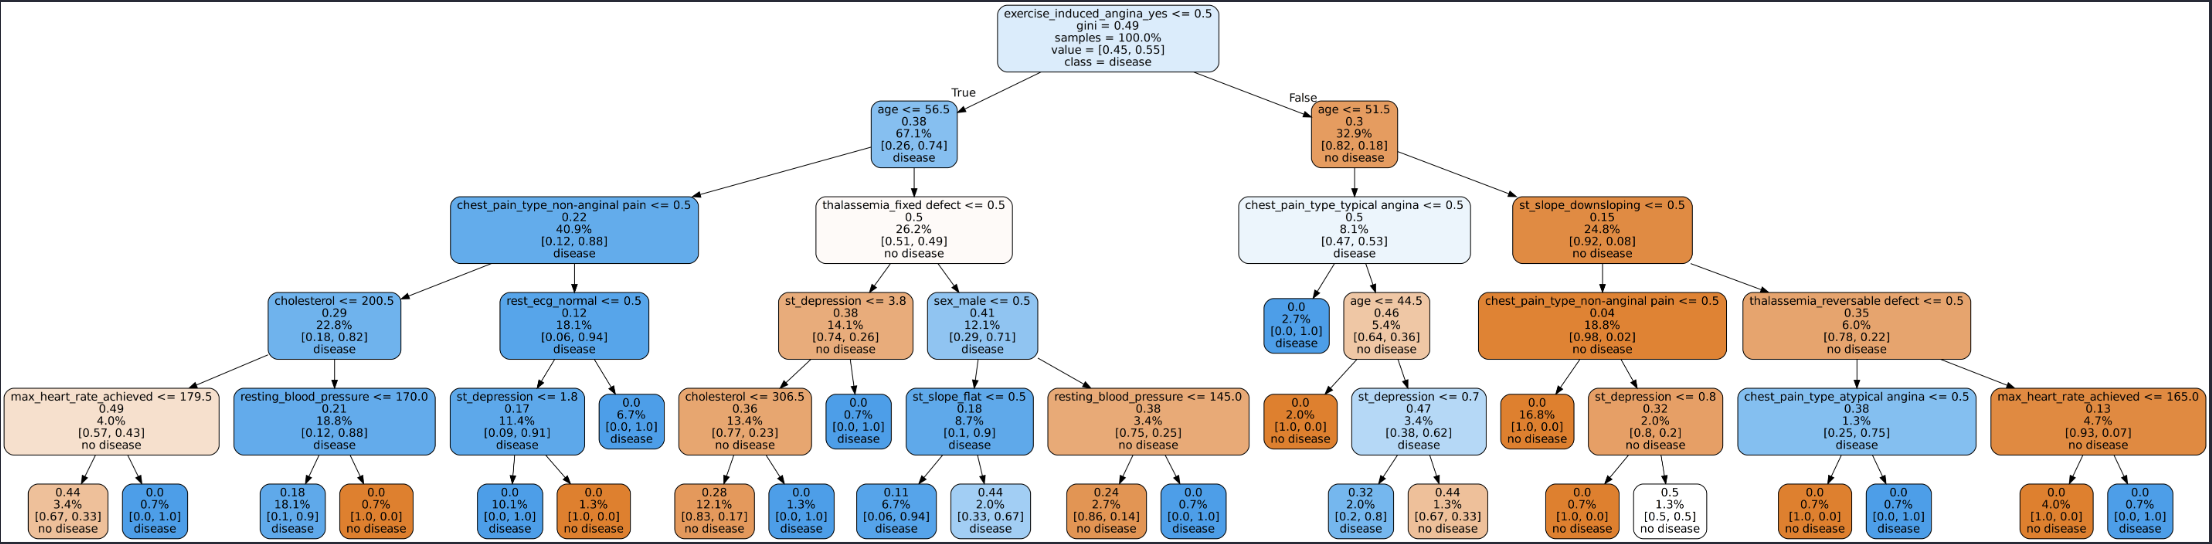
\includegraphics[width=1.0\textwidth]{portfolio/Decision_Tree.png}
        % 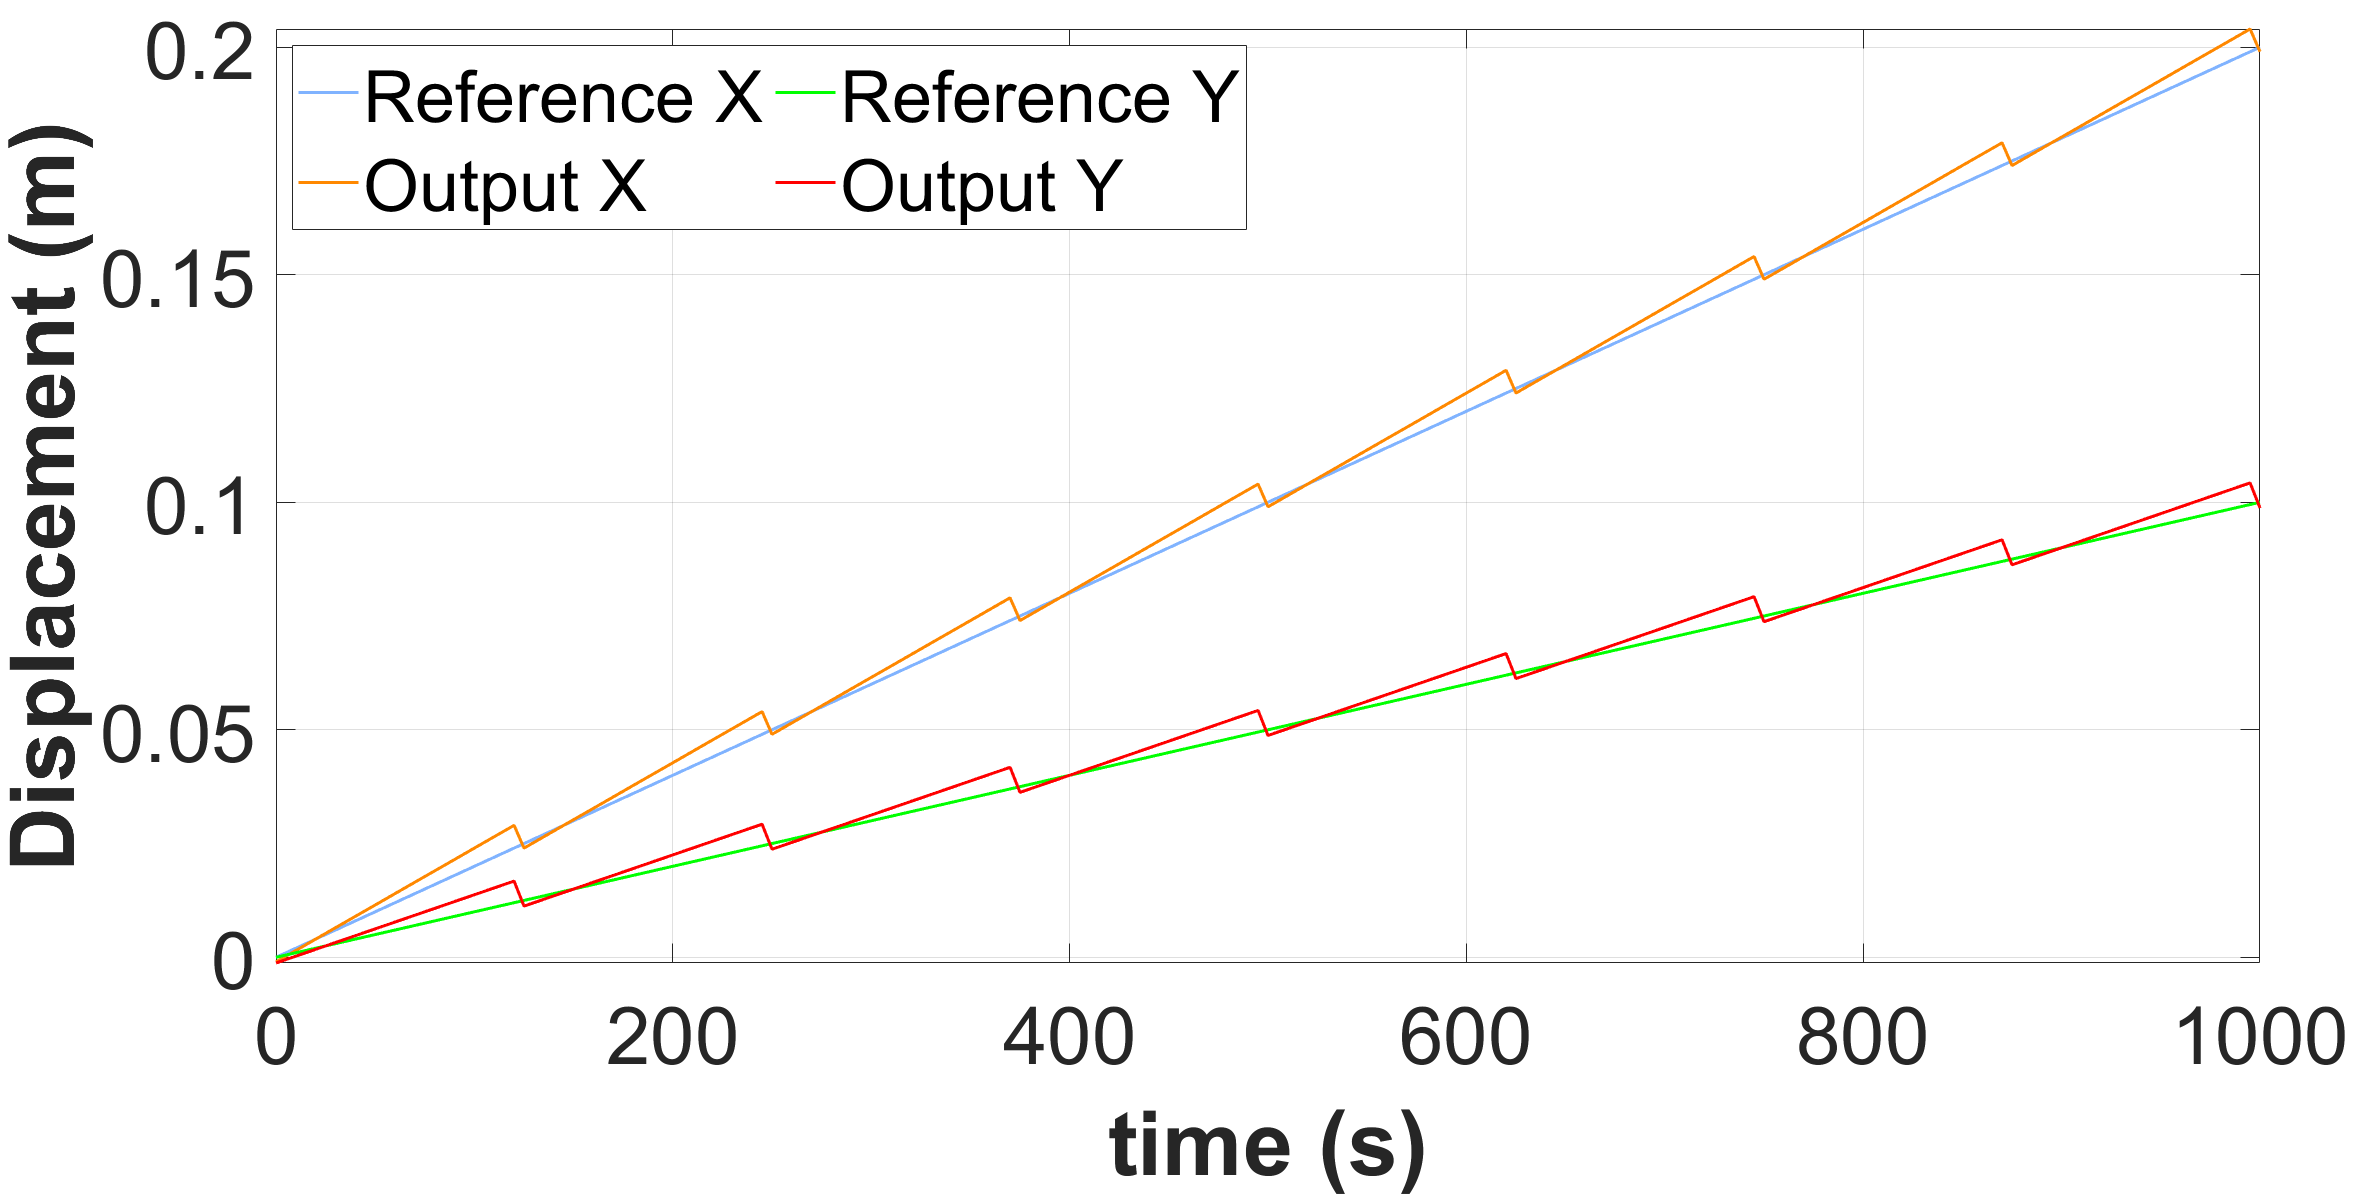
\includegraphics[width=0.45\textwidth]{portfolio/feedforward_track.png}
        \caption{Decision Tree of Random Forest Model}
        \label{Random Forest Model}
    \end{figure}

    \item {Evaluation of the prediction success rate, shown in Figure \ref*{Model-Evaluation}}
    \begin{figure}[H]
        \centering
        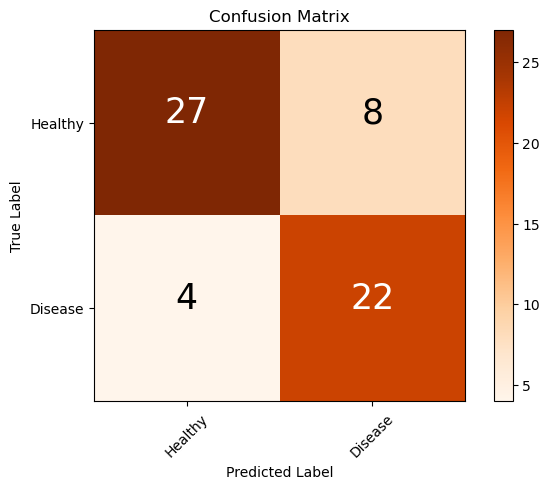
\includegraphics[width=0.45\textwidth]{portfolio/Confusion_Matrix.png}
        % 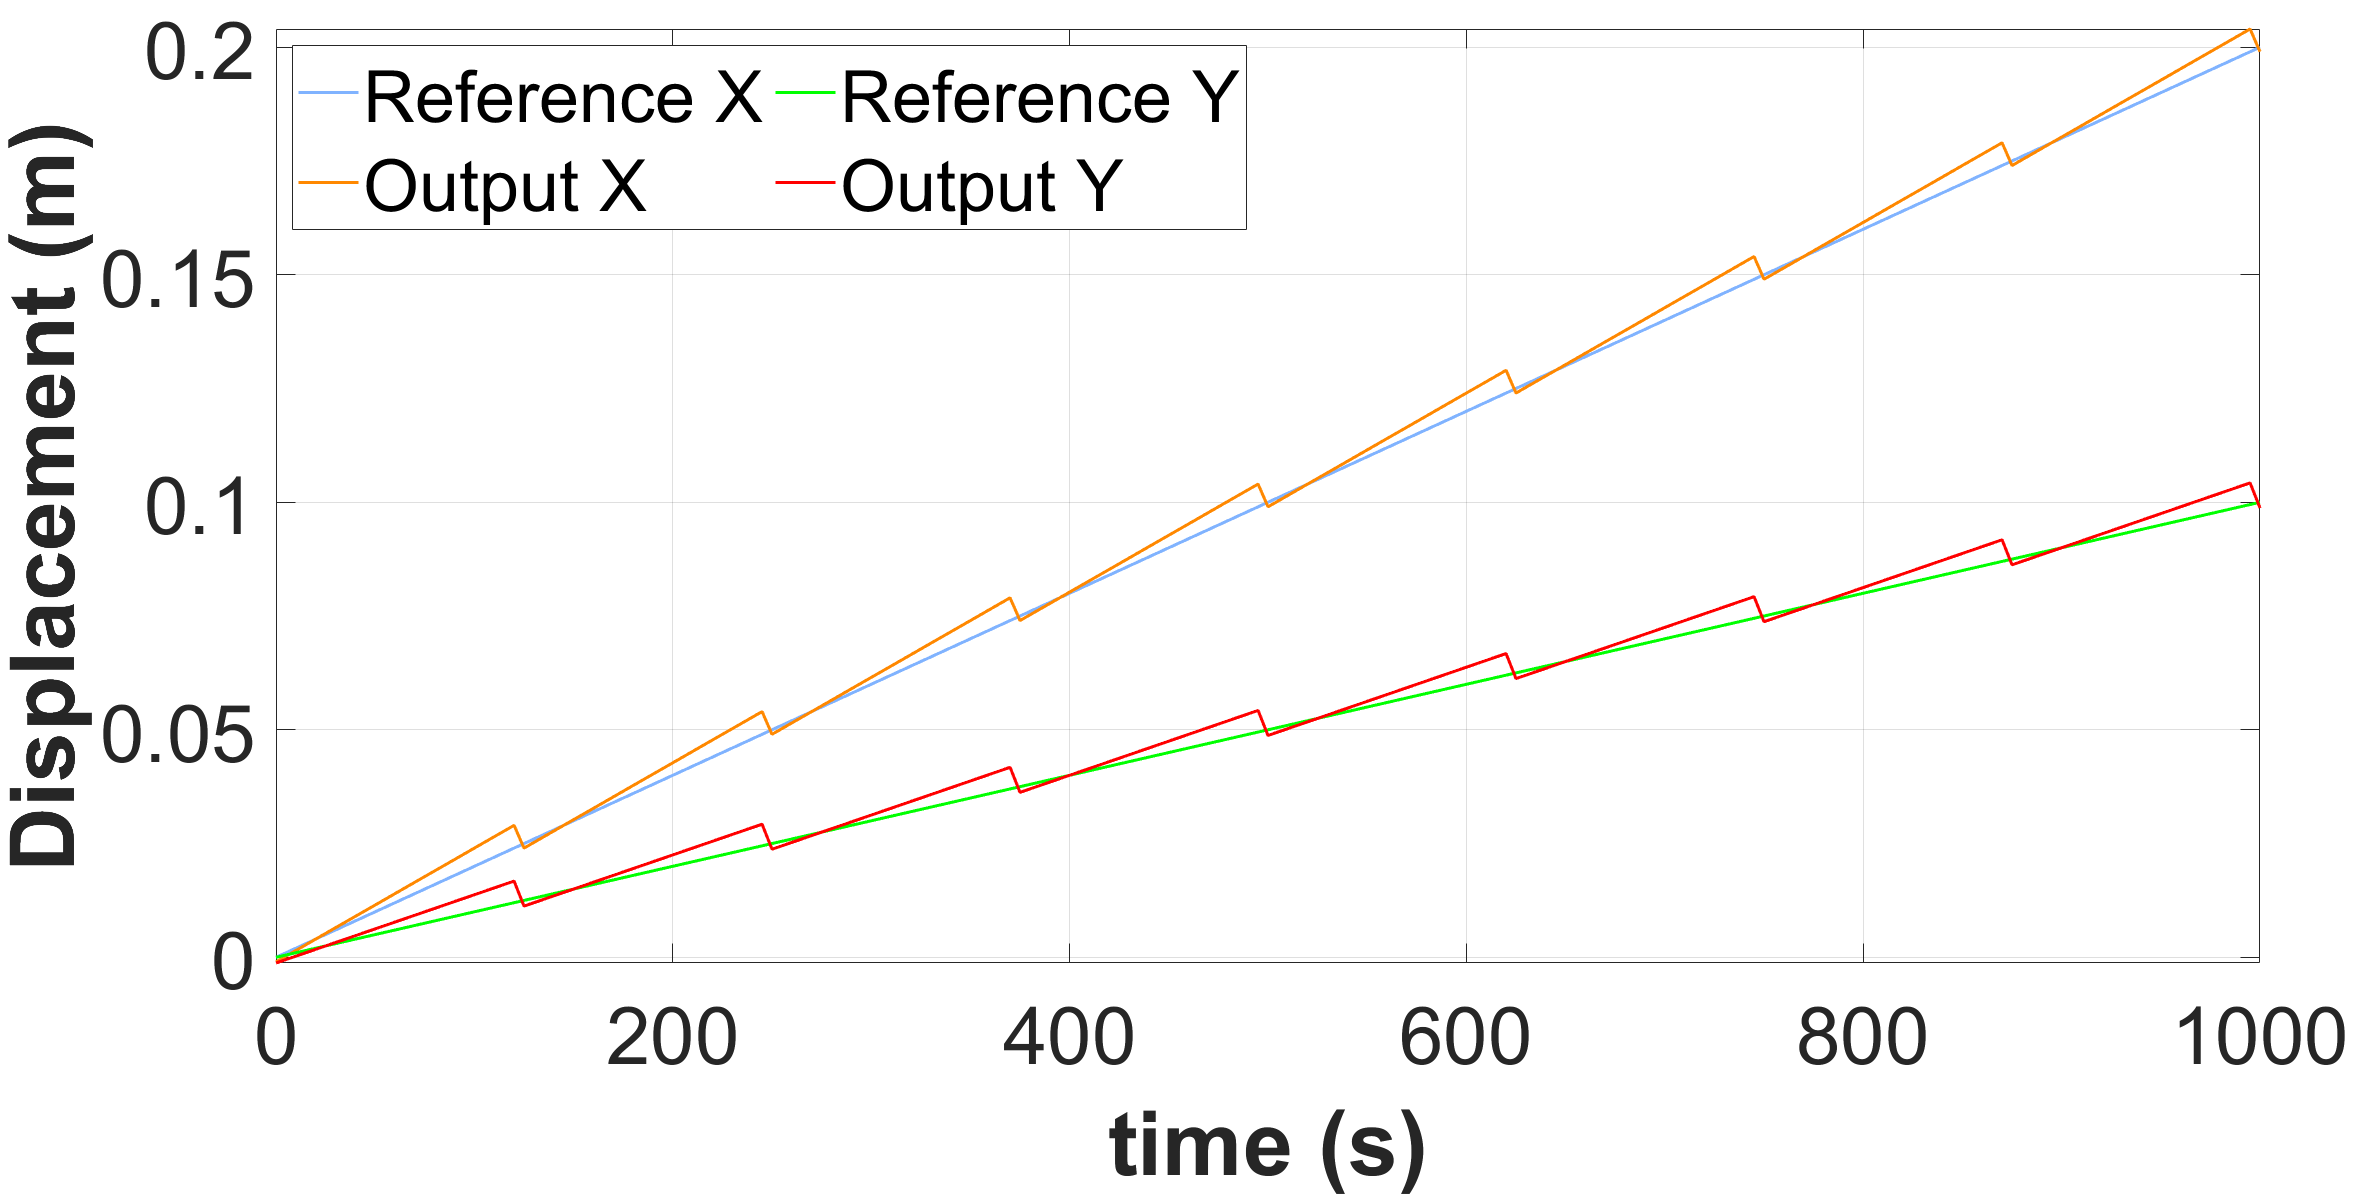
\includegraphics[width=0.45\textwidth]{portfolio/feedforward_track.png}
        \caption{Prediction Result of Classification Model by Confusion Matrix}
        \label{Model-Evaluation}
    \end{figure}
    
\end{itemize}

\newpage

\section{Automated Vehicle with Tracking System}

\subsection{Objectives}

\begin{enumerate}

    \item {Design and control of the gimbal stabilizer, which processes the estimation of distance and deviation angle from the camera module.}
    \item {Build communication portal among the gimbal stabilizer, the the camera module, and the central controller for cruise control.}

\end{enumerate}

\subsection{Results}

\begin{itemize}

    \item {A gimbal stabilizer to stabilize the camera module and performs object tracking, as shown in Figure \ref*{Stabilizer-Control}.}
    \begin{figure}[H]
        \centering
        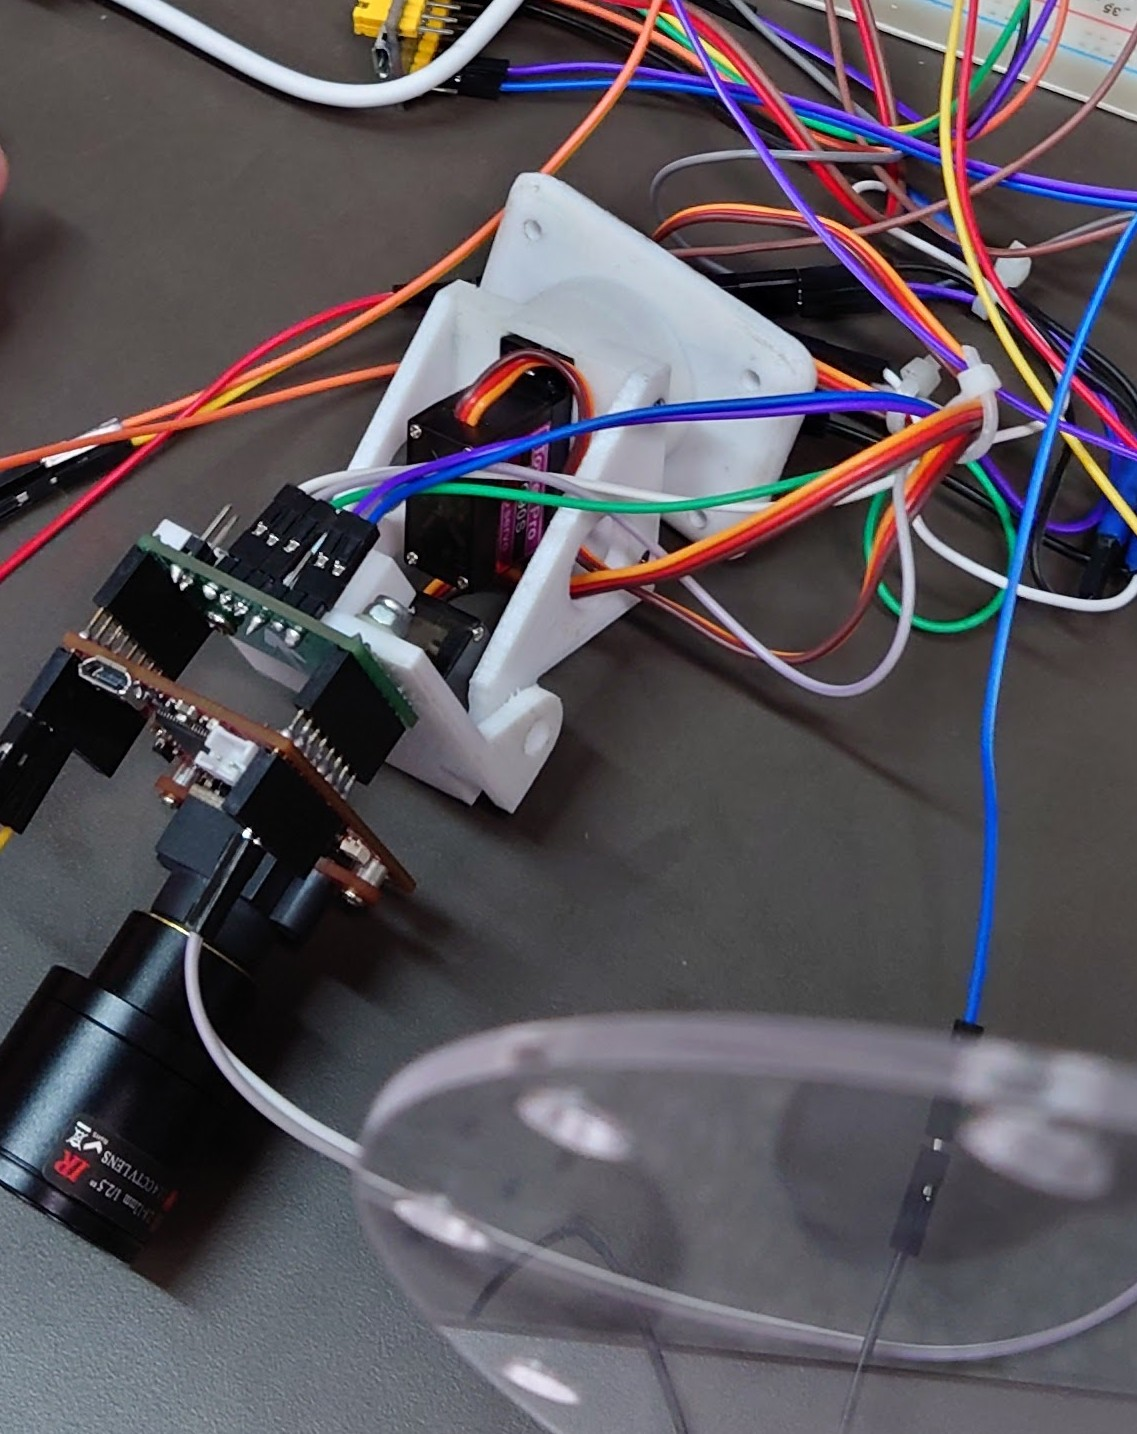
\includegraphics[width=0.45\textwidth]{portfolio/Gimbal.JPG}
        % 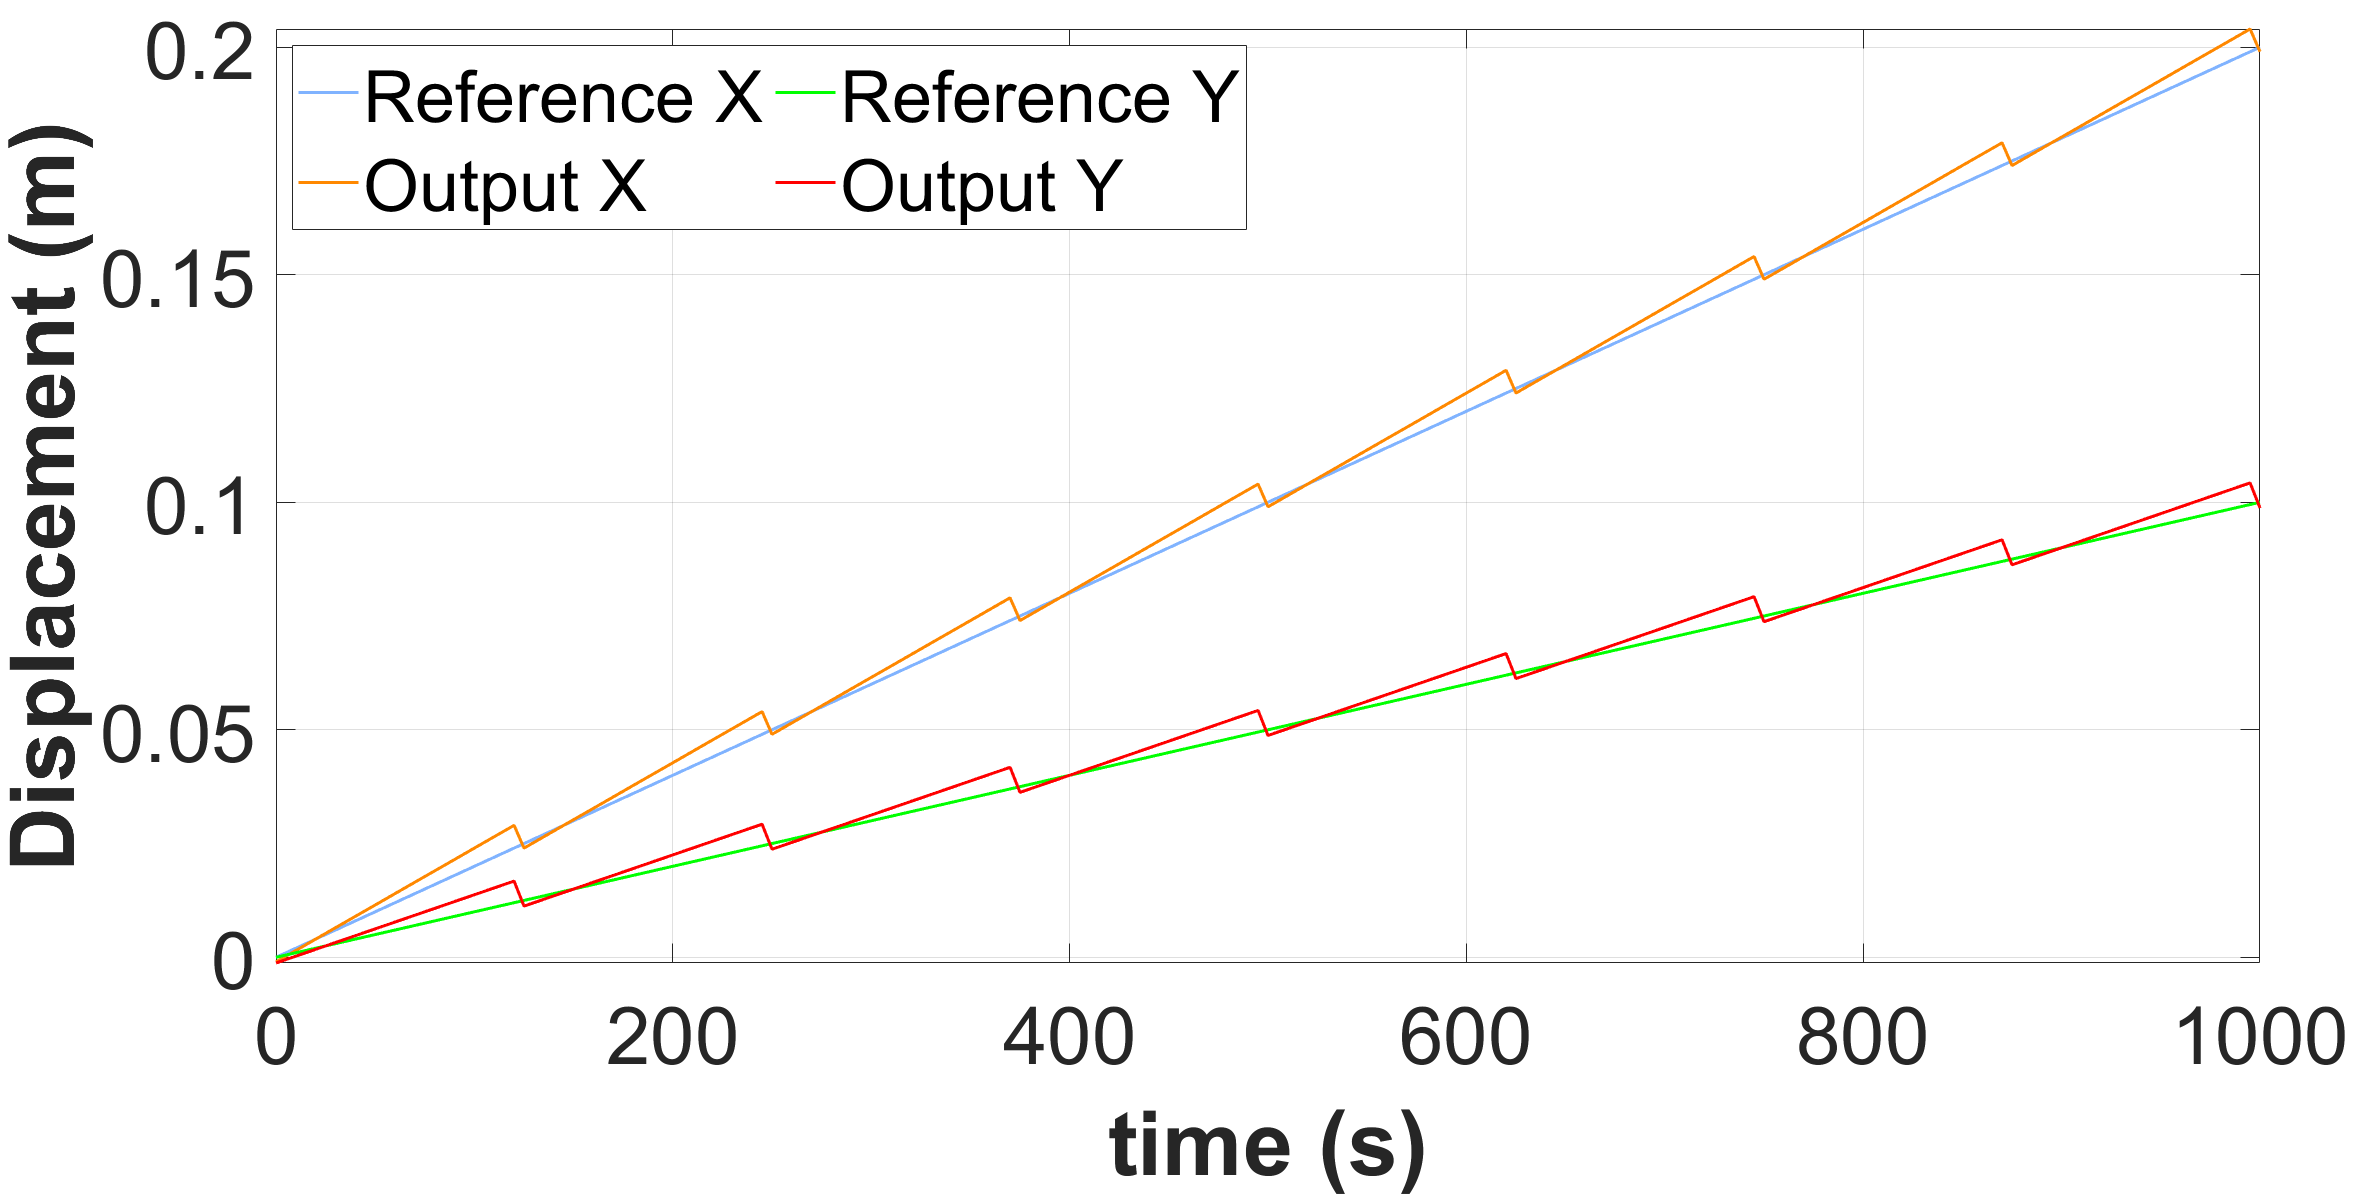
\includegraphics[width=0.45\textwidth]{portfolio/feedforward_track.png}
        \caption{Gimbal Stabilizer}
        \label{Stabilizer-Control}
    \end{figure}
    \item {Control strategies applied to the gimbal stabilizer,  \href{https://github.com/Robin0265/StablerCTRL}{GitHub Repo}}
\end{itemize}

% % -- END OF DOC -- % 
\end{document}